\documentclass[../../main.tex]{subfiles}

\begin{document}
        \subsubsection*{Shimming}

            Durch Ausführung des automatischen Shimming Bisektionsalgorithmus der Prospa Software \cite[ch. 2.4.3]{doc:EFNMRStudentManual} erhalten wir in $36$ Iterationen mit einer Schrittgröße von $0.00975\si{\milli\ampere}$ in einer Zeitspanne von $4:49$min unter noch nicht vollständig optimierten Parametern der $B_1$ Pulsdauer $t_{B_1}$ [siehe Kap. \ref{subsubsec:5:B1PulsdauerOptimierung}] und der Kapazität $C$ [siehe Kap. \ref{subsubsec:5:Kapazitaetsoptimierung}] die in Tabelle \ref{tab:5:AutoShimParameter} dargestellten richtungsabhängigen Werte. Dabei verwenden wir ein von der Anleitung abweichendes, relativ schmales Suchintervall von $2\si{\milli\ampere}$ mit einer in der Anleitung angegebenen Abbruchbedingung von $0.1\si{\milli\ampere}$ \cite[ch 2.4.3]{doc:EFNMRStudentManual}. 

            \begin{table}[H]
                \centering
                \begin{tabular}{|c|c|c|}
                    \hline
                    $x$ & $y$ & $z$ \\
                    \hline\hline
                    $-3.99\si{\milli\ampere}$ & $-28.84\si{\milli\ampere}$ & $3.83\si{\milli\ampere}$
                    \\\hline
                \end{tabular}
                \caption{Zum Richtungsgradienten des Shimmingmagnetfeldes korrespontierende Parameter in $[\si{\milli\ampere}]$.}
                \label{tab:5:AutoShimParameter}
            \end{table}
            Die ausführlicheren Pulse Sequence Parameter sind in der Konfigurationsabbildung \ref{fig:5:AutoShimKonfiguration} dargestellt. Betrachtet man das Amplitudenverhalten während des Prozesses, so erkennt man bereits relativ optimal gewählte Startwerte, da ein deutlicher Amplitudenanstieg pro Iteration ausbleibt und teilweise sogar wieder abfällt, bei einer Standardabweichung von $\sigma = 1.33\si{\micro\volt}$ um den Mittelwert $\overline A = 38.52\si{\micro\volt}$. 
            \begin{figure}[H]
                \centering
                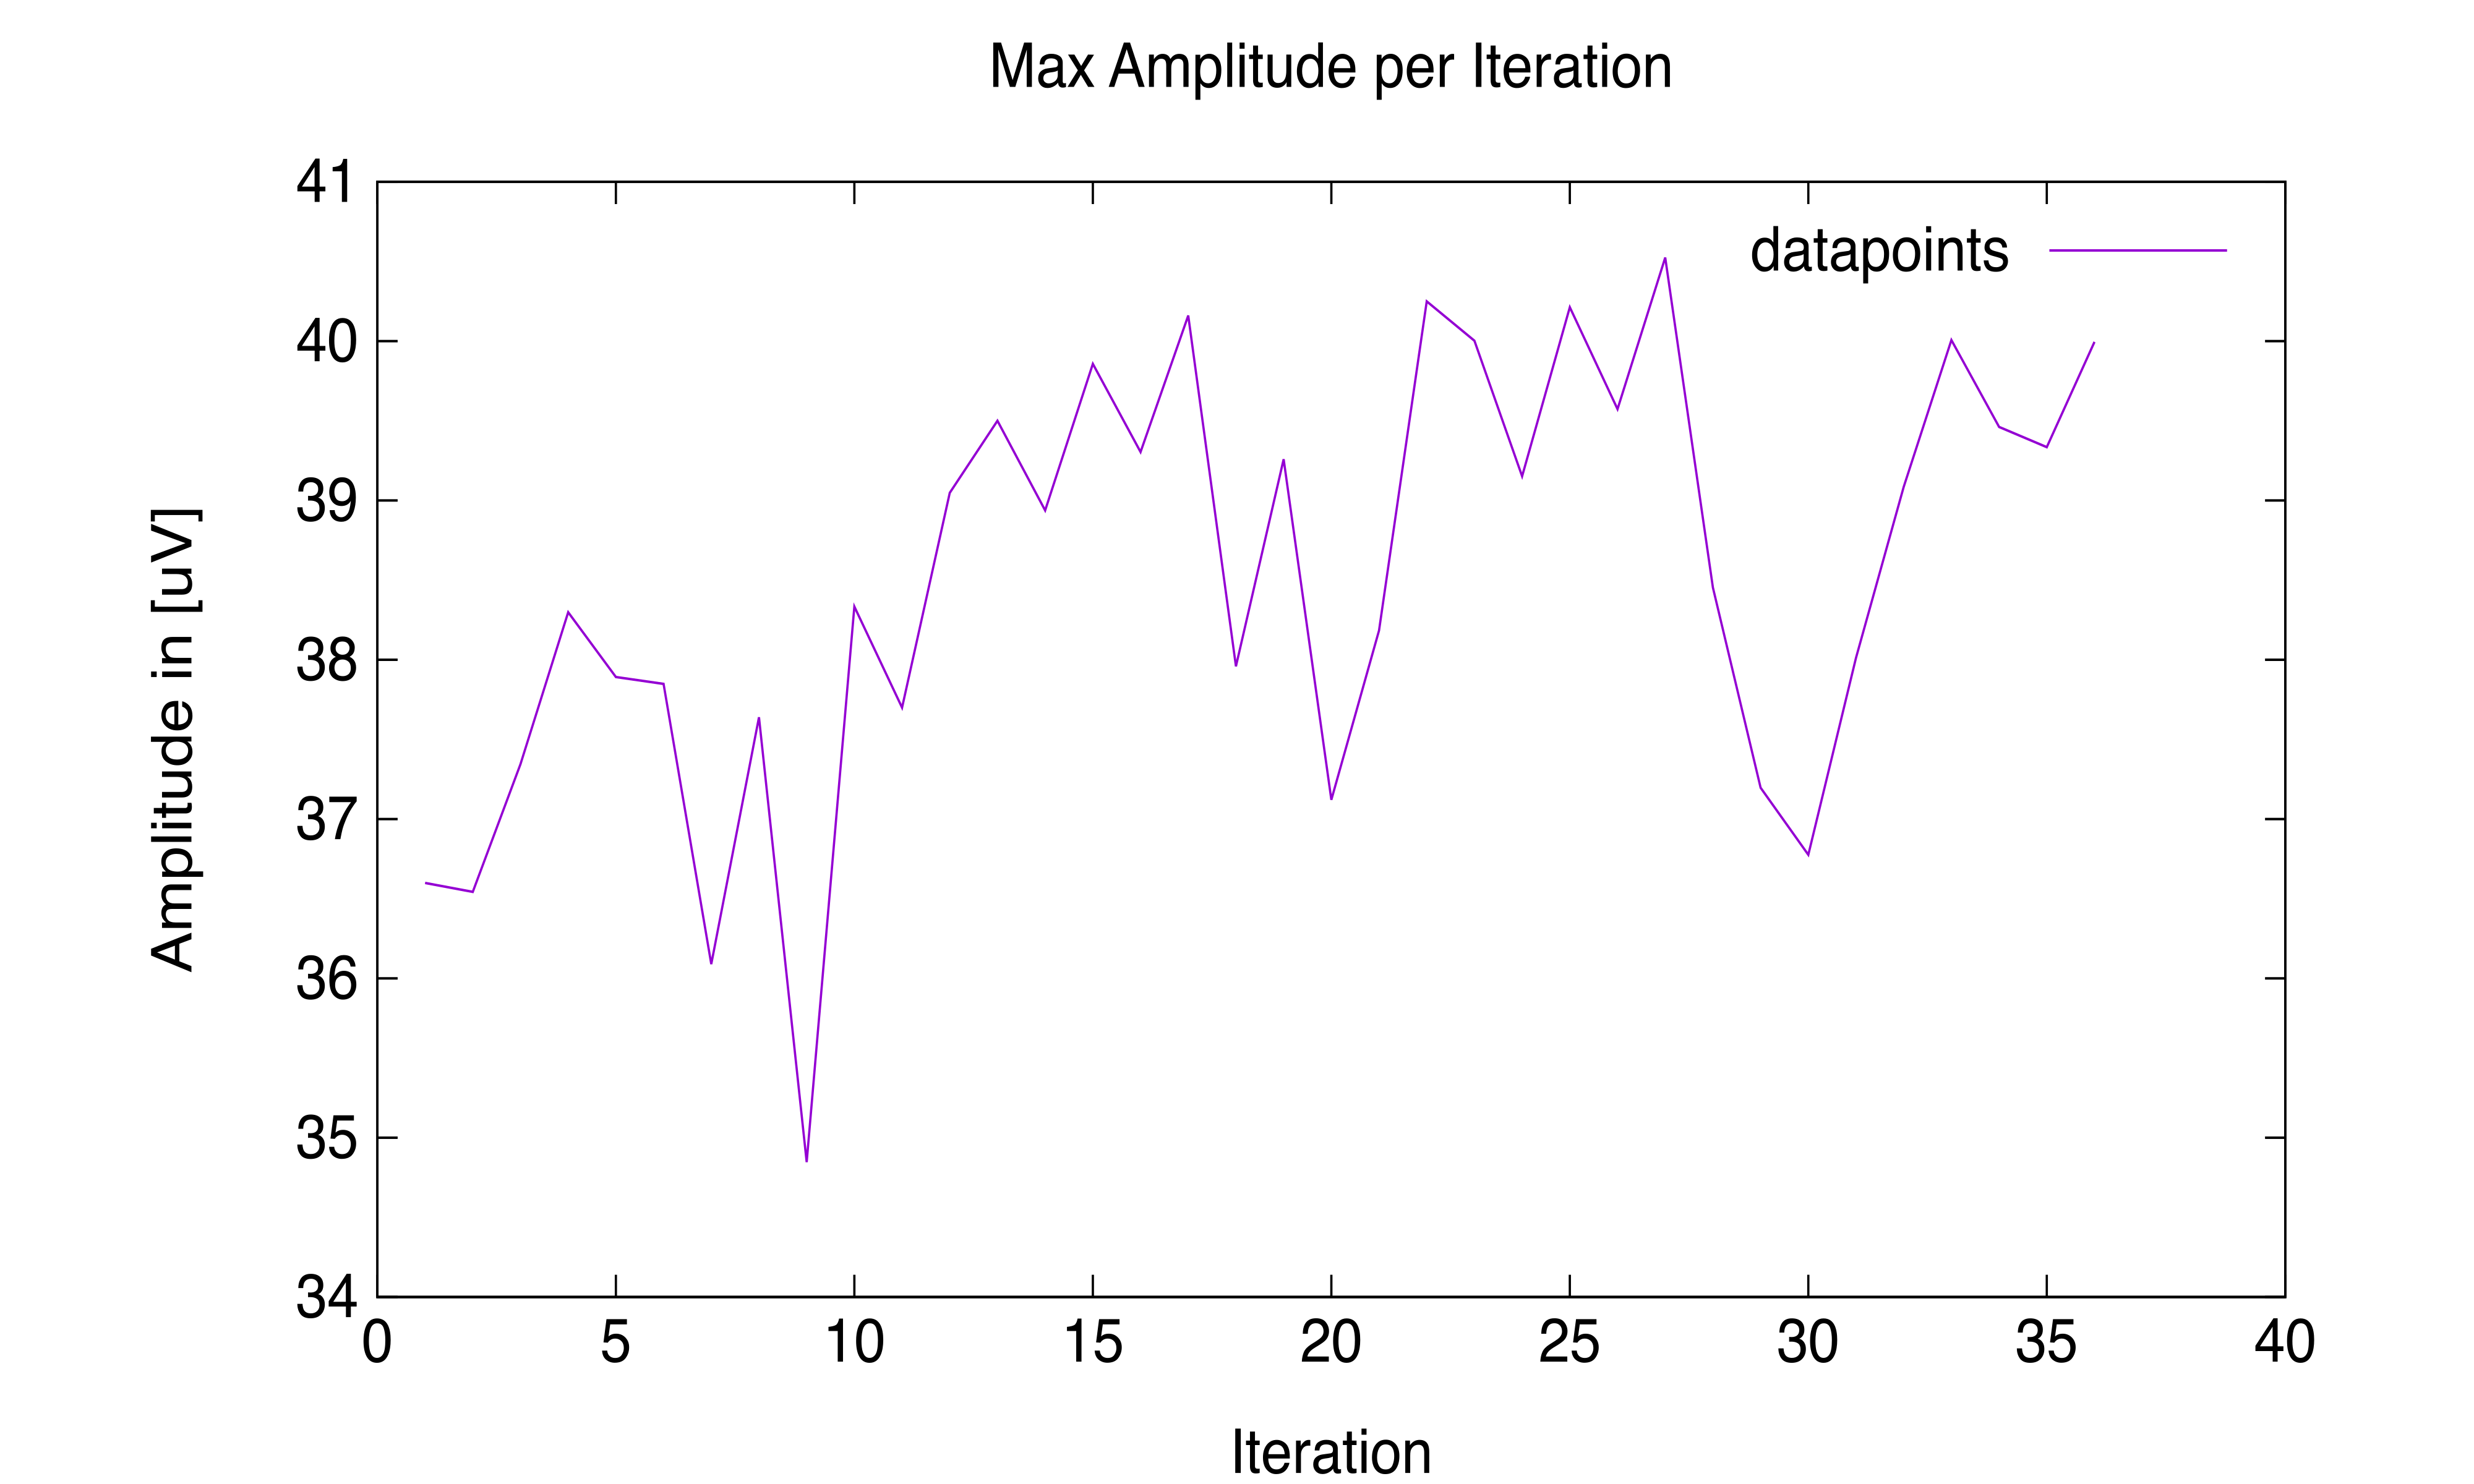
\includegraphics[width=11cm]{Bilddateien/5/AutoShim2_Iteration.png}
                \caption{Amplitudenverlauf während des automatischen Shimmings.}
                \label{fig:5:AutoShimAmplitudenverlauf}
            \end{figure}
            Dabei sind bei der Messung des FID und Berechnung des zugehörigen Spektrums die gewünschten Formen deutlich erkennbar [siehe Abb. \ref{fig:5:AutoShimFIDSpectrum}], was auf ein erfolgreiches Shimming hinweist.
            \begin{figure}
                \centering
                \begin{subfigure}[t]{0.45\textwidth}
                    \centering
                    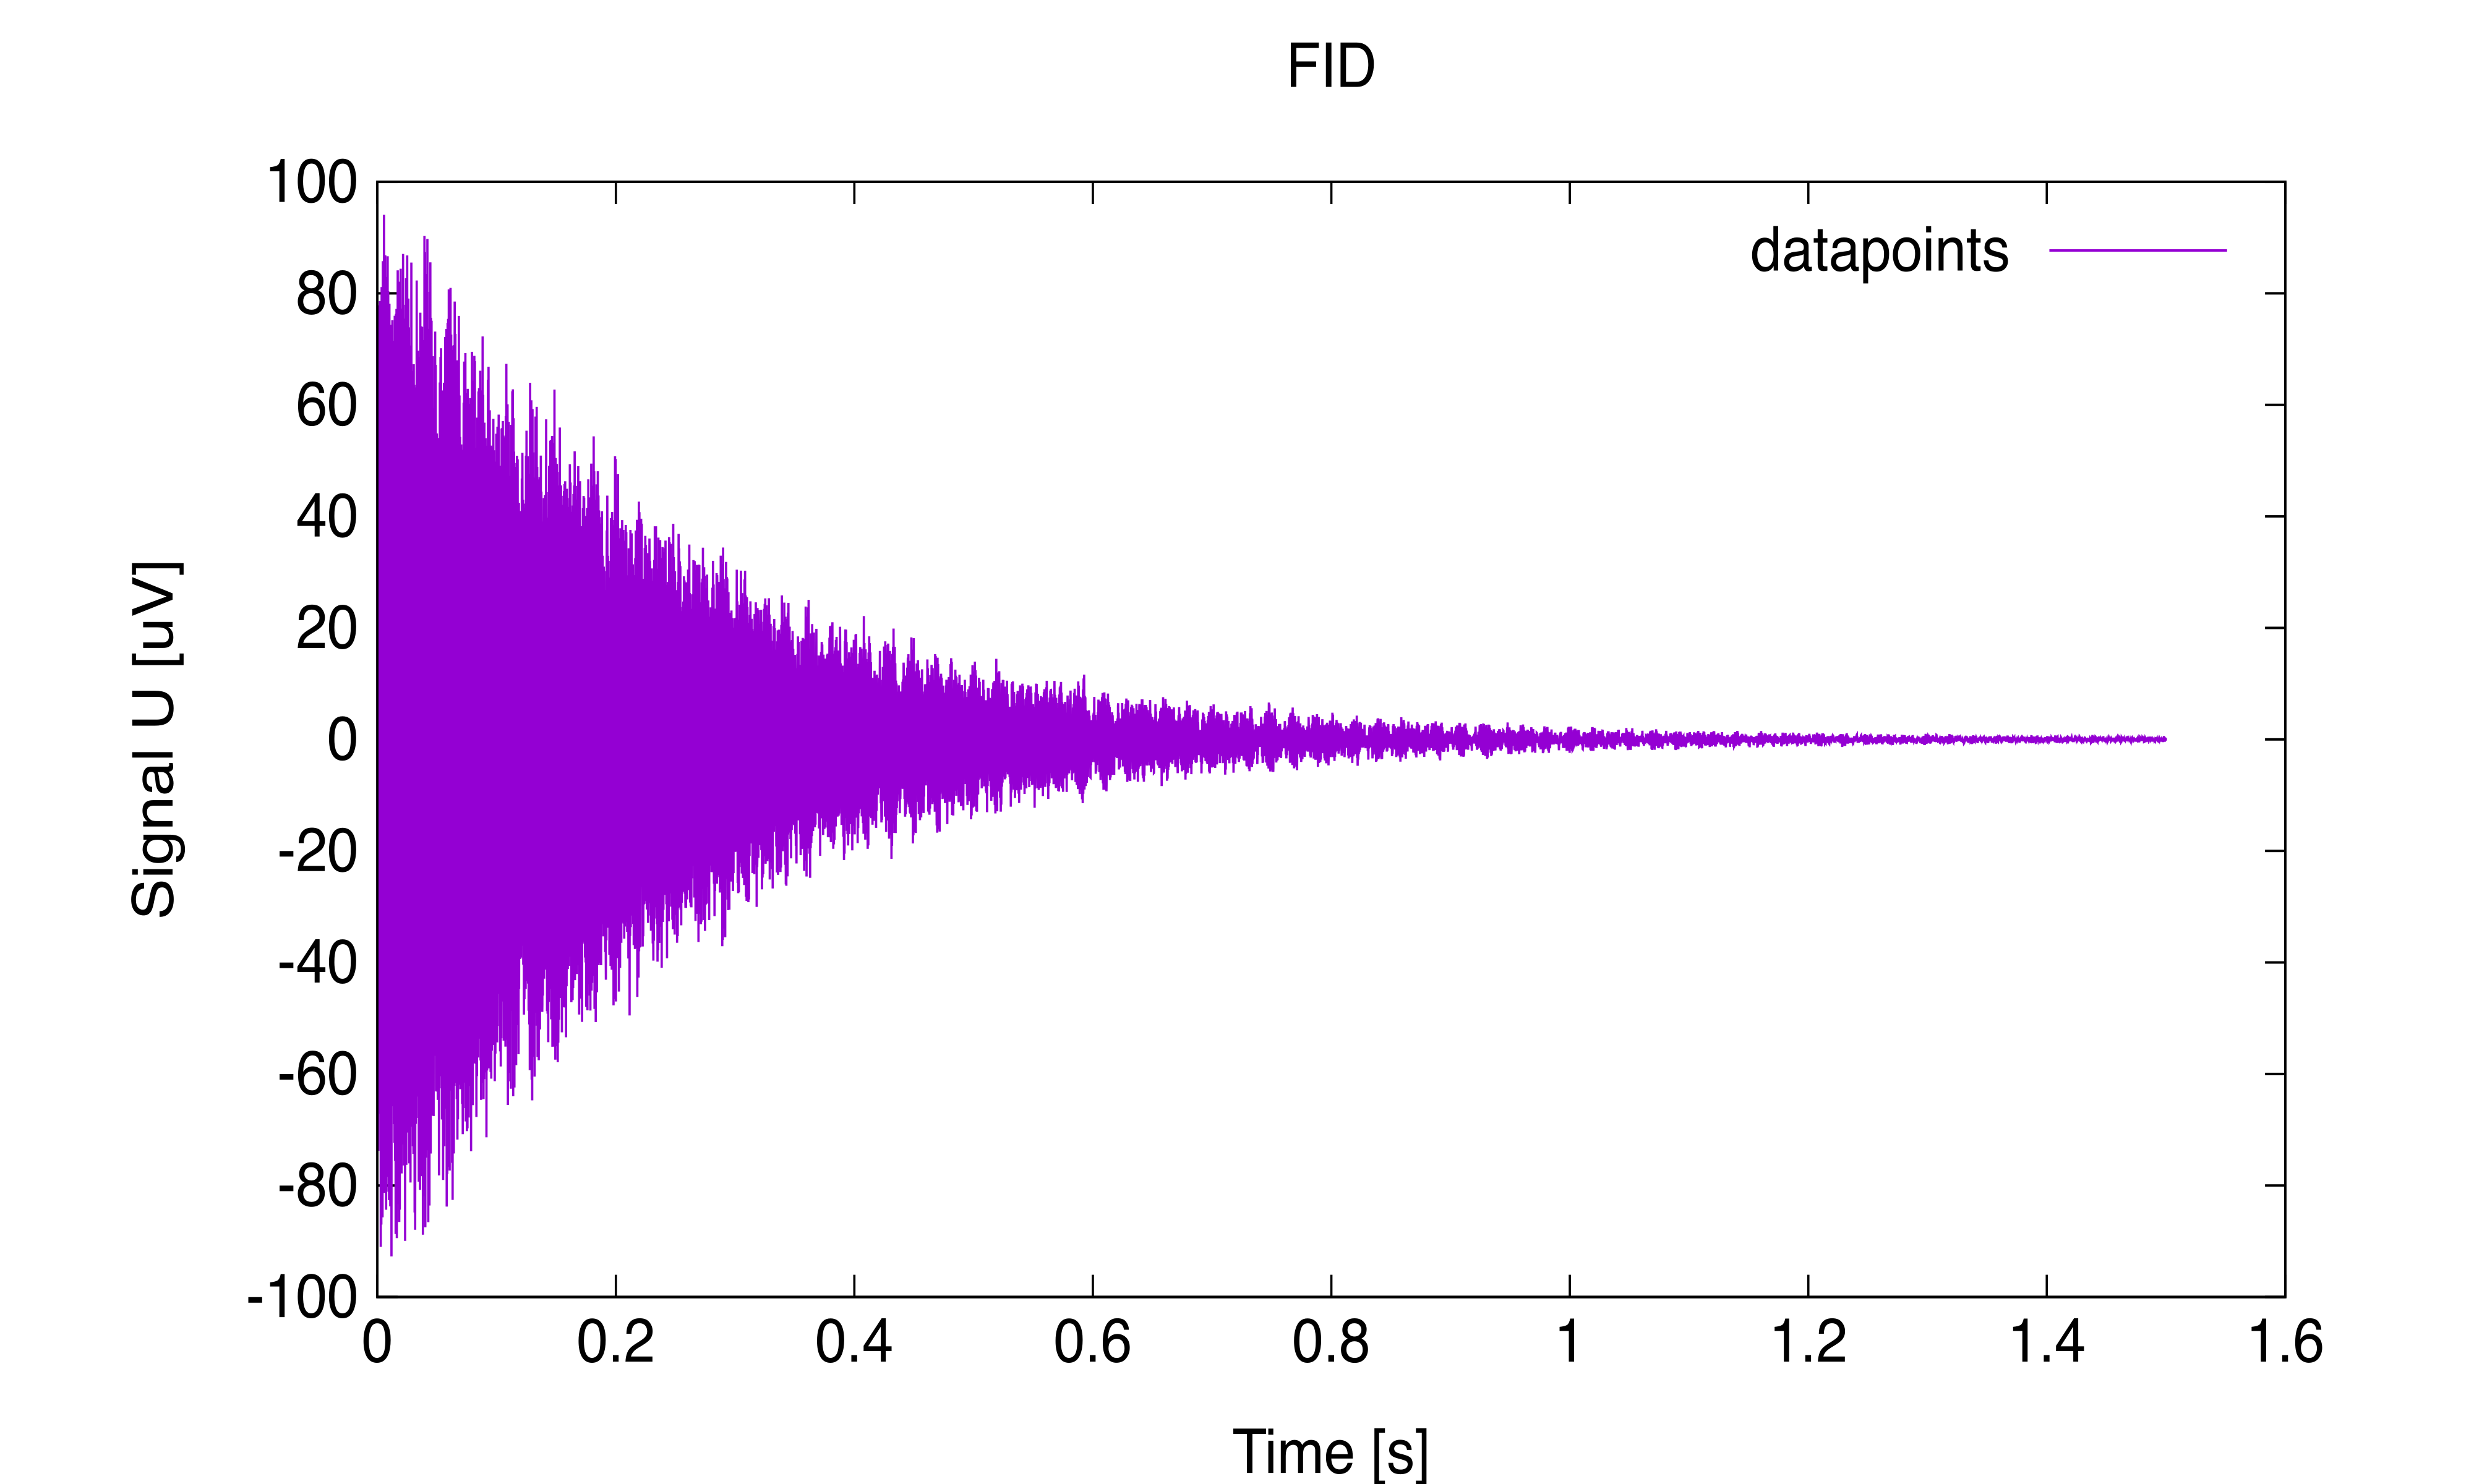
\includegraphics[width=6cm]{Bilddateien/5/AutoShim2_FID.png}
                    \caption{FID.}
                \end{subfigure}
                \
                \begin{subfigure}[t]{0.45\textwidth}
                    \centering
                    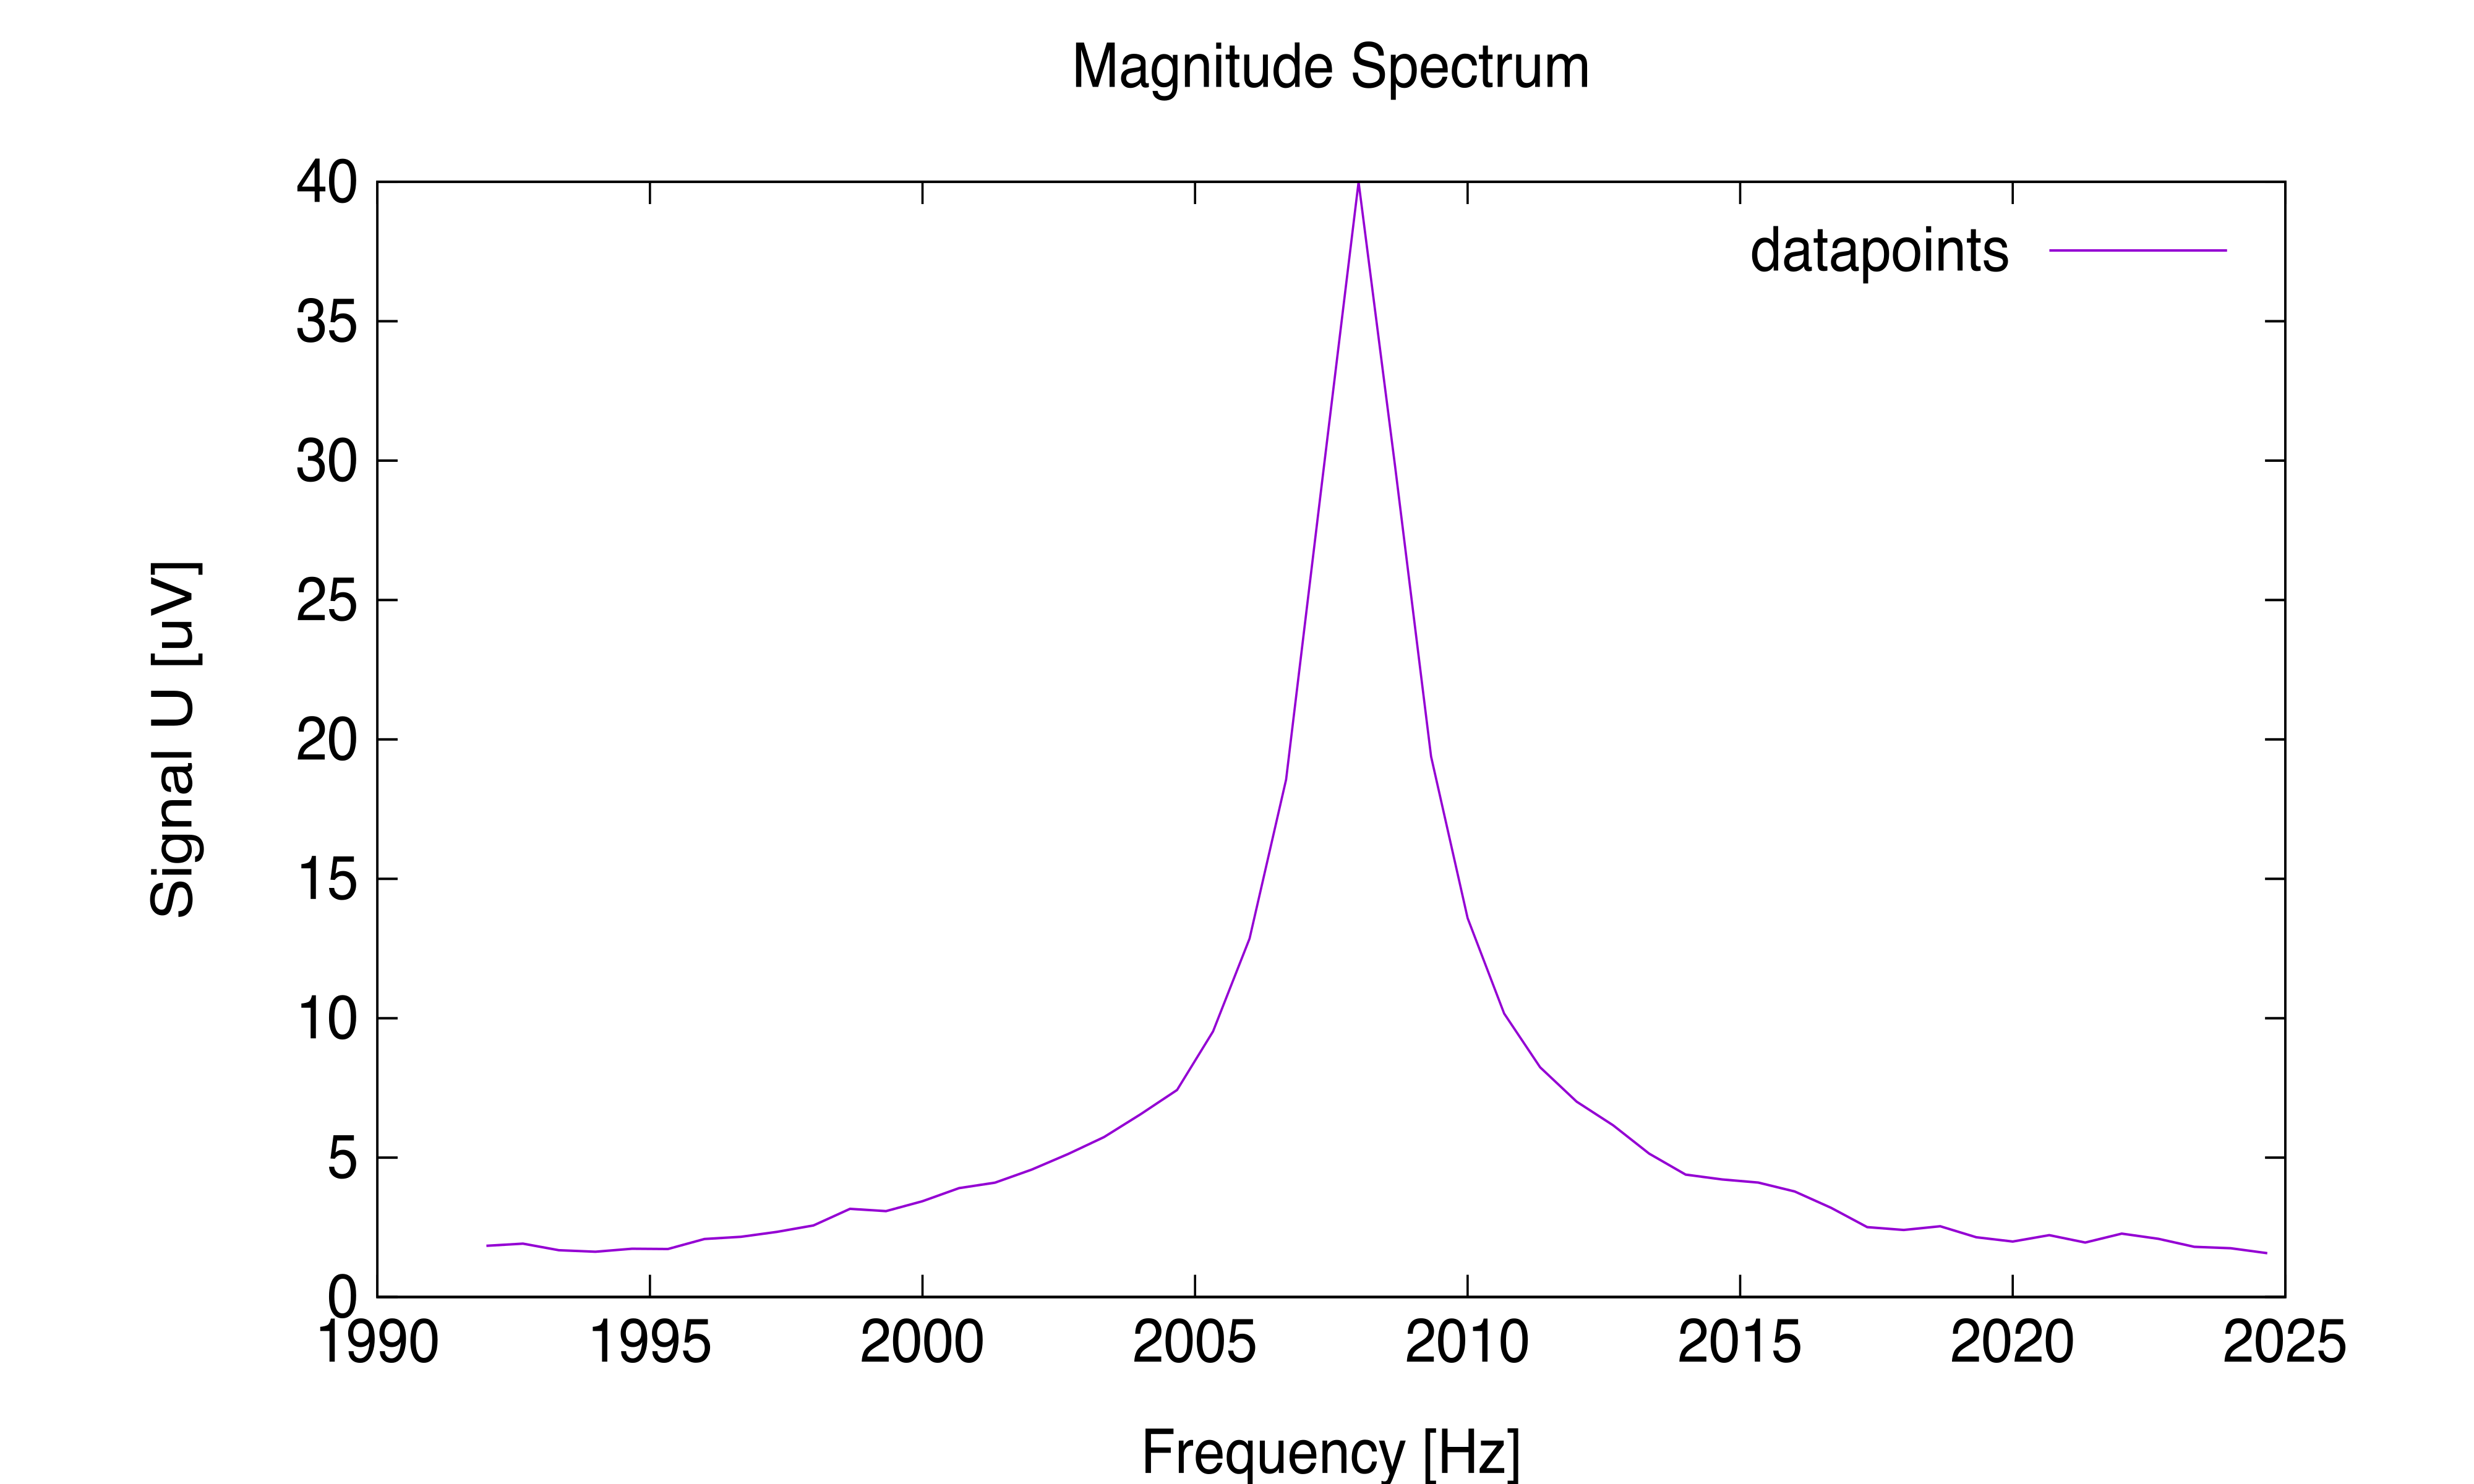
\includegraphics[width=6cm]{Bilddateien/5/AutoShim2_Spectrum.png}
                    \caption{Spektrum.}
                \end{subfigure}
                \caption{FID und Spektrum nach automatischem Shimming.}
                \label{fig:5:AutoShimFIDSpectrum}
            \end{figure}

            \begin{figure}[H]
                \centering
                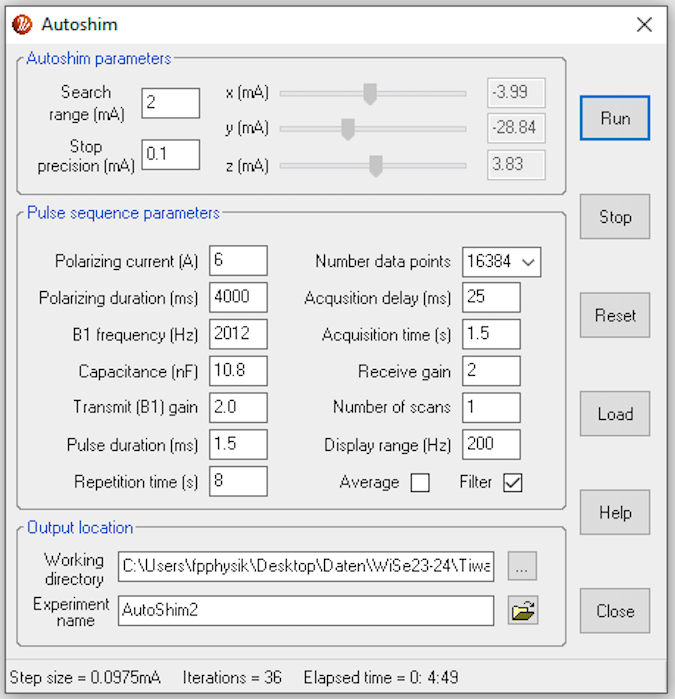
\includegraphics[width=7cm]{Bilddateien/5/AutoShim_Konfigurationsparameter.png}
                \caption{Konfiguration der automatischen Shimming Pulse Sequence.}
                \label{fig:5:AutoShimKonfiguration}
            \end{figure}

        \subsubsection*{Kapazitätsoptinierung}\label{subsubsec:5:Kapazitaetsoptimierung}
            Die Optimierung der LCR-Schwingkreiskapaizität $C$ erfolgt bei uns lediglich durch optische Analyse des Larmor-Peakverhaltens und der LCR-Schwingkreisresonanz. Wir stützen uns auf die Berechnung aus Kapitel \ref{subsec:4:LCRResonanzanalyse} und den bereits voreingestellten Wert von $10.8\si{\nano\farad}$. Aufgrund der optisch ausreichenden Übereinstimmung der beiden Frequenzen, wie in Abbildung \ref{fig:5:OptiCSpectrum} ersichtlich, entscheiden wir uns für die Verwendung des voreingestellten Wertes.
            \begin{figure}[H]
                \centering
                \begin{subfigure}[t]{0.45\textwidth}
                    \centering
                    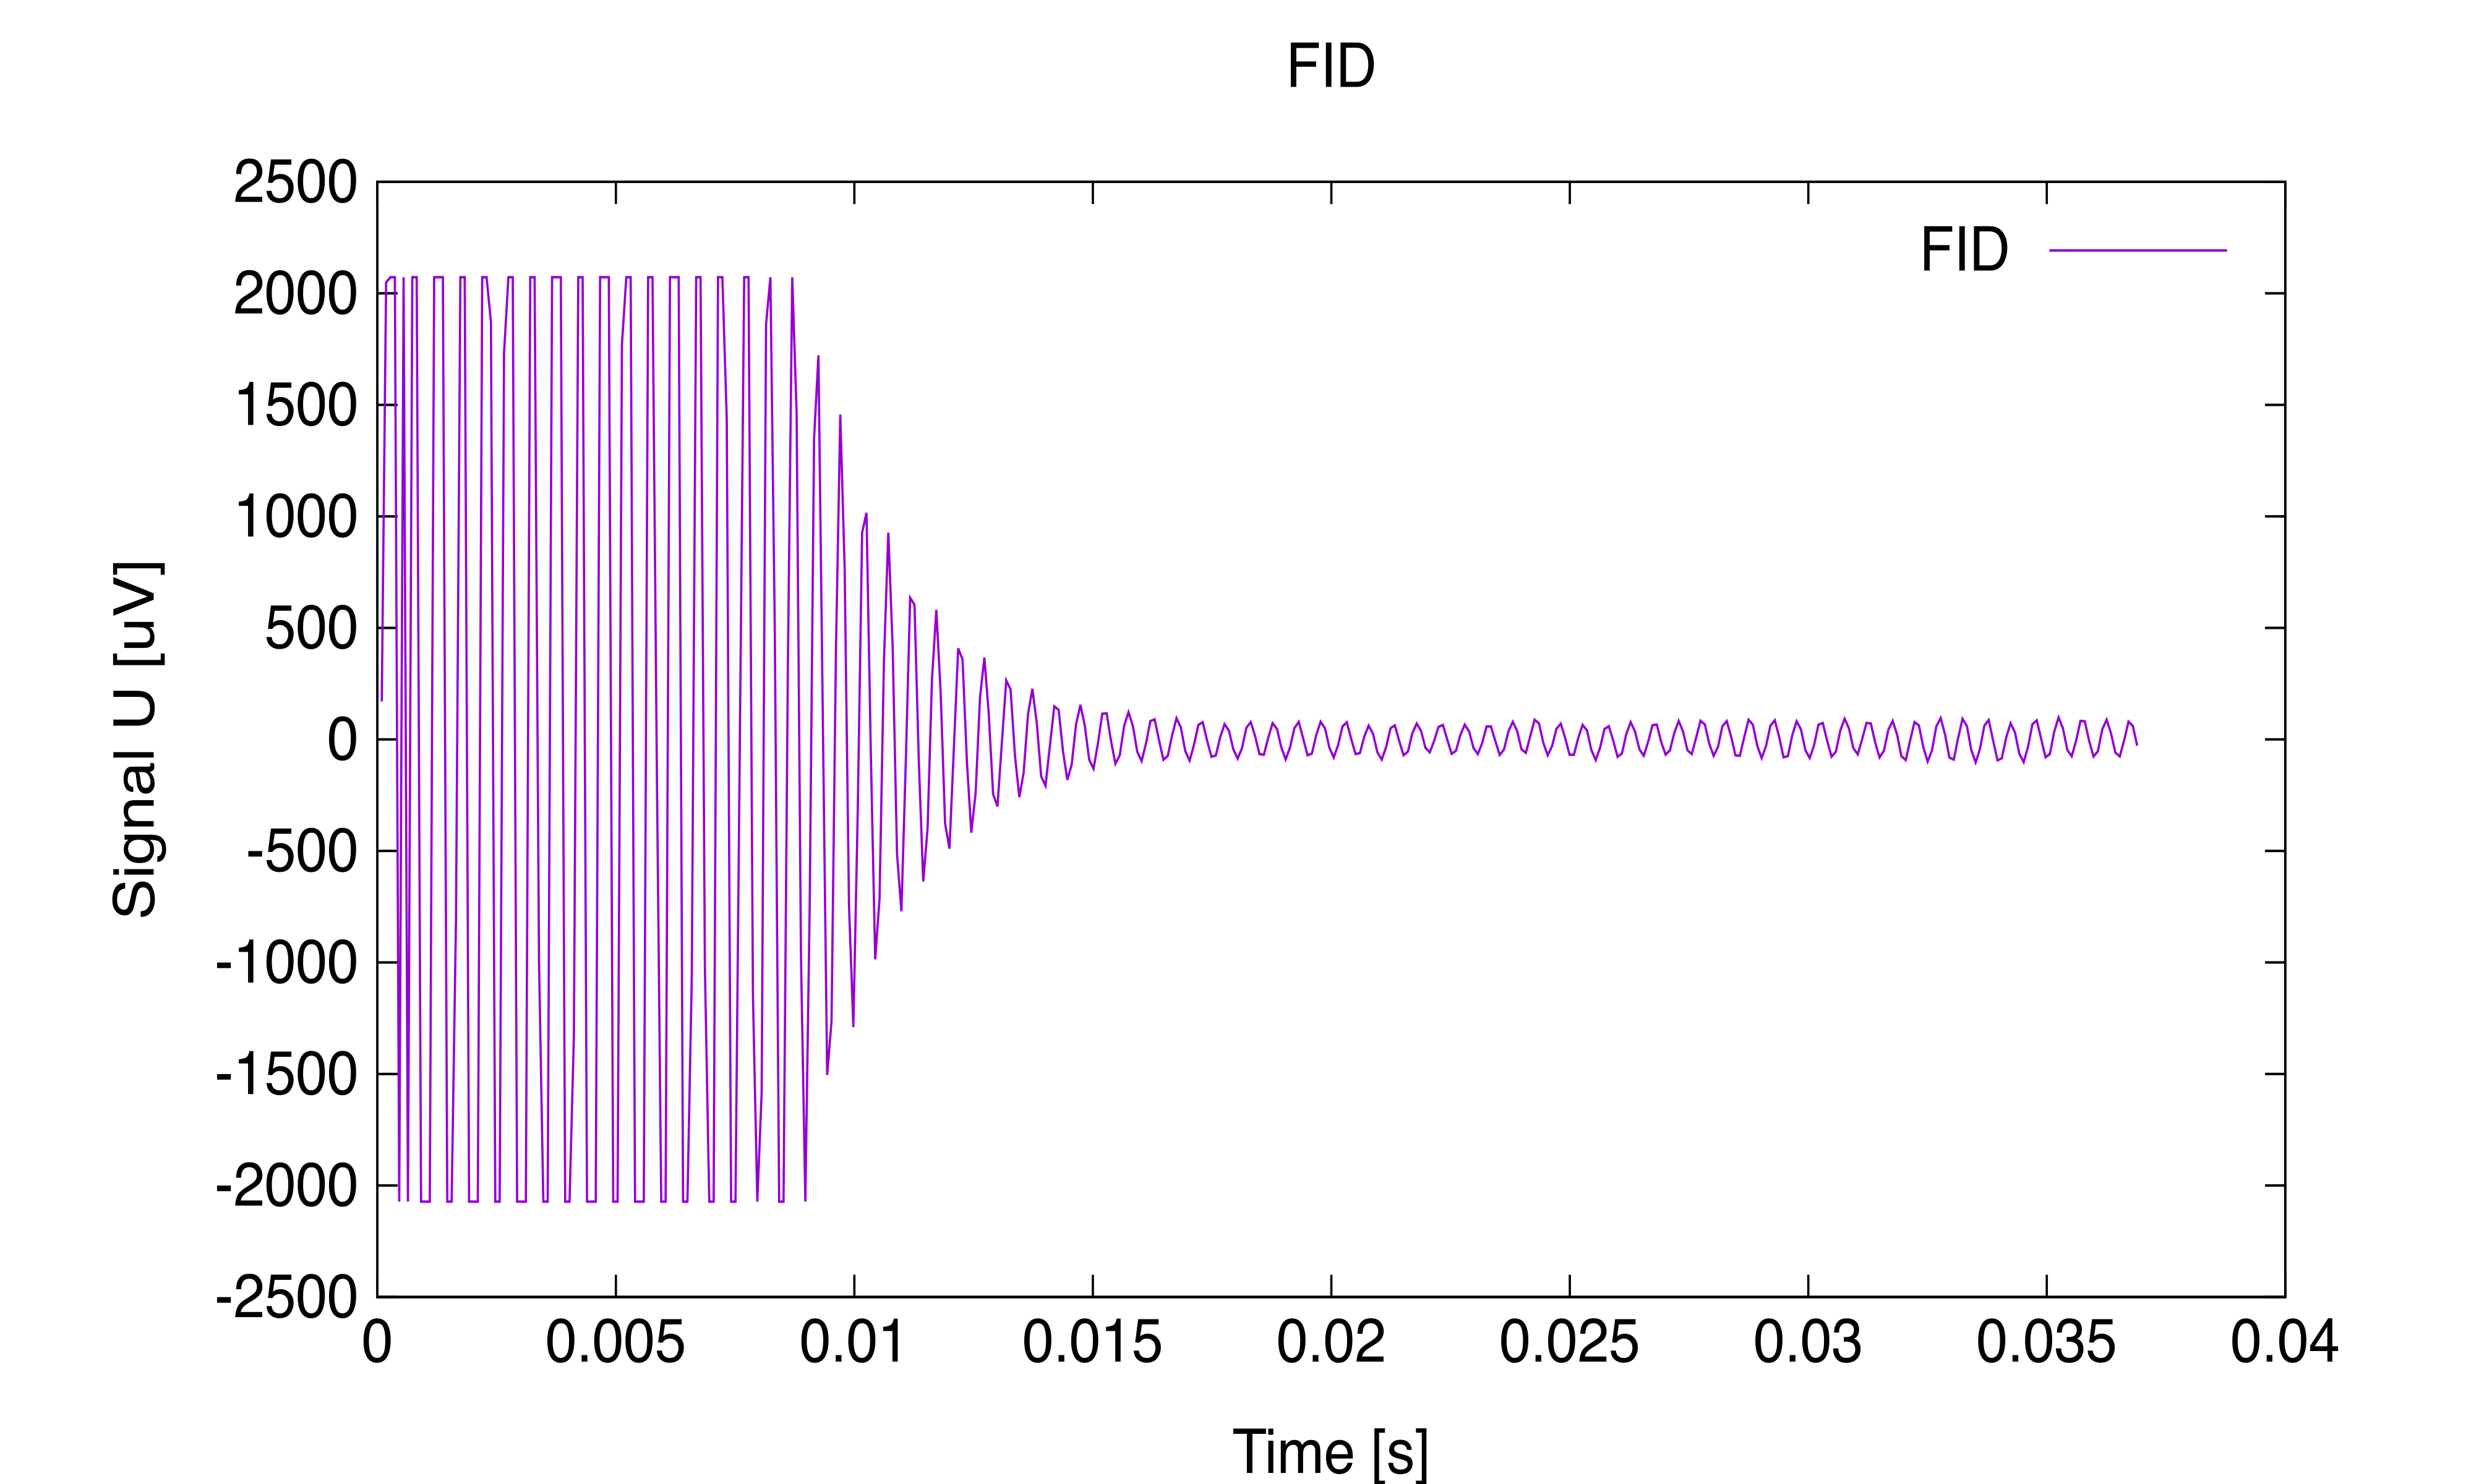
\includegraphics[width=6cm]{Bilddateien/5/C_Opti_FID.png}
                    \caption{Messung der FID-Amplitude mit optimierter Kapazität.}
                \end{subfigure}
                \
                \begin{subfigure}[t]{0.45\textwidth}
                    \centering
                    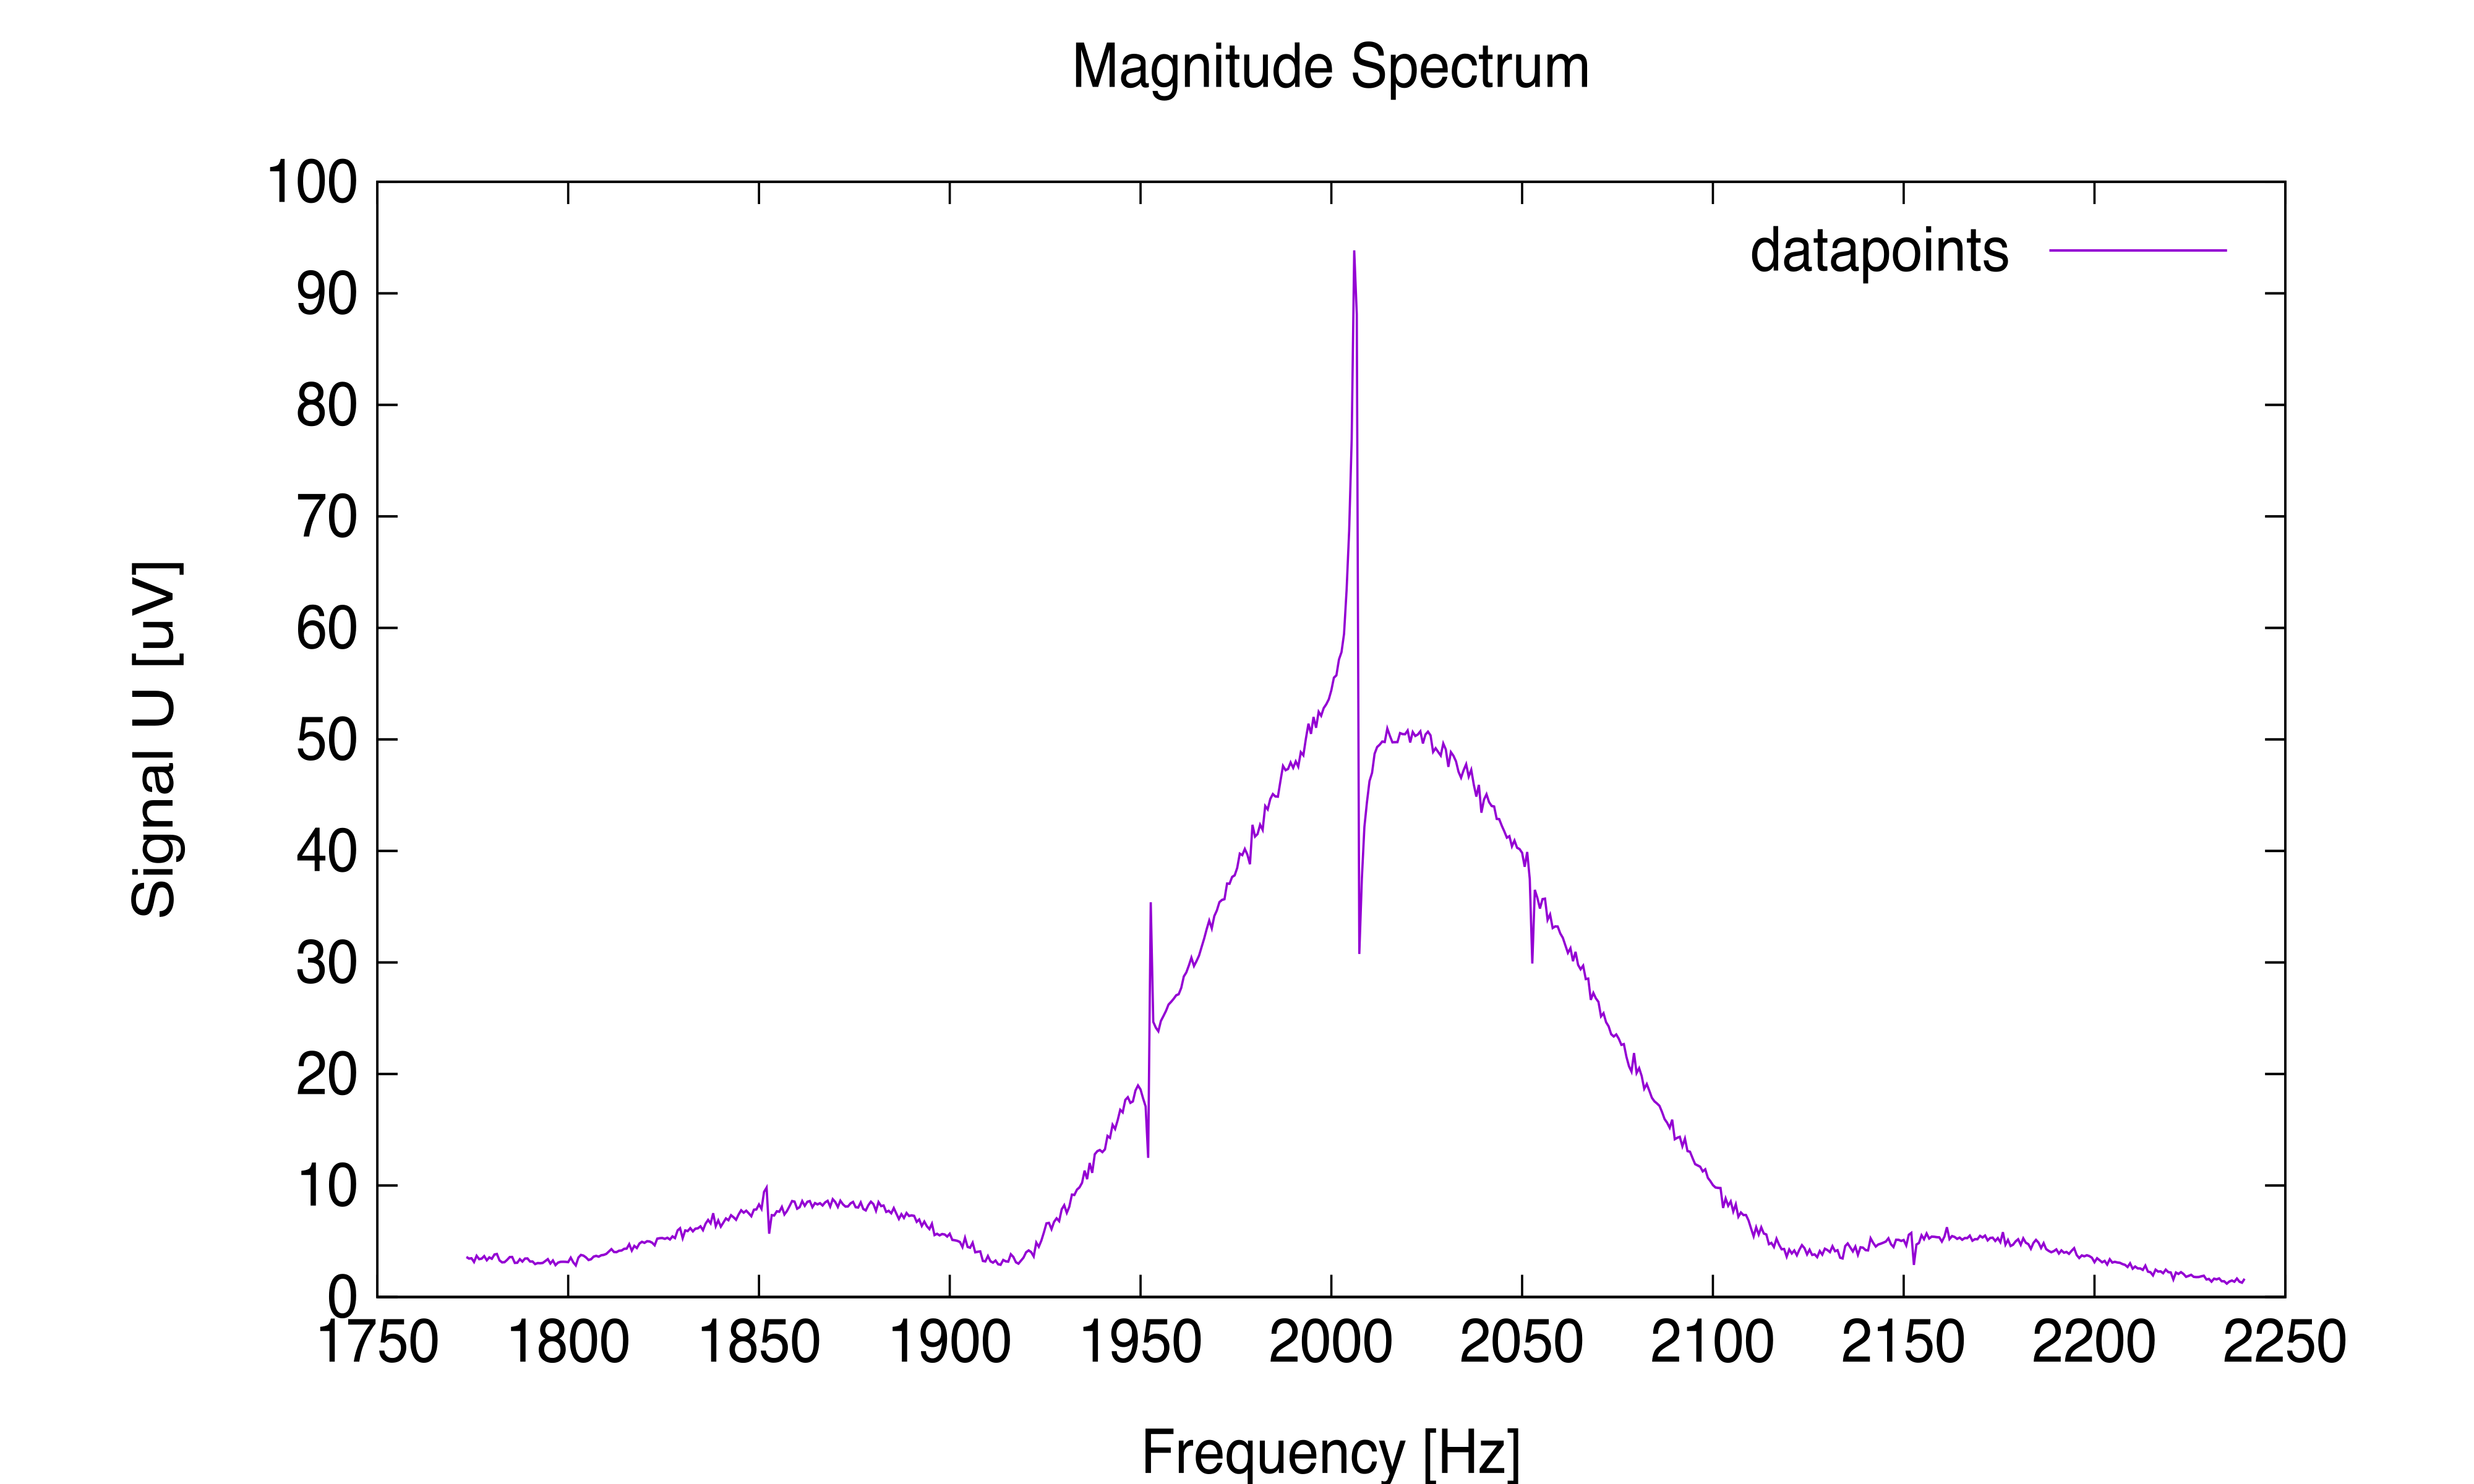
\includegraphics[width=6cm]{Bilddateien/5/C_Opti_Spectrum.png}
                    \caption{Messung des Spektrums mit optimierter Kapazität.}
                    \label{subfig:5:OptiCSpectrum}
                \end{subfigure}
                \caption{Messung der FID-Amplitude und des Spektrums mit optimierter Kapazität.}
                \label{fig:5:OptiCSpectrum}
            \end{figure}
            Deutlich erkennbar ist die Larmor-Frequenz im optischen Zentrum des Resonanzpeaks des LC-Schwingkreises als Interferenz des scharfen Resonanzpeaks der Nukleonen mit dem einer sinc Funktion folgenden Verlauf der LCR-Schwingkreisresonanz. Ihre Form ist dabei dem Effekt des sogenannten \enquote{coil ring downs} unter Fouriertransformation zuzuschreiben, unter welchem der Abklang der Resonanzreaktion des Schwingkreises über die Zeit verstanden wird \cite[ch 1.4.5]{doc:EFNMRStudentManual}. In unserem Experiment verwenden wir hier eine Zeitverzögerung der Messung von voreingestellten $2\si{\ms}$. Unsere verwendeten Parameter stellen wir in Abbildung \ref{fig:5.1:B1OptiParameter} aus. Die erkennbaren Nebenpeaks erklären wir uns durch die in Kapitel \ref{subsec:3:Rauschanalyse} bereits diskutierten Oberschwingungen. 
            \begin{figure}[H]
                \centering
                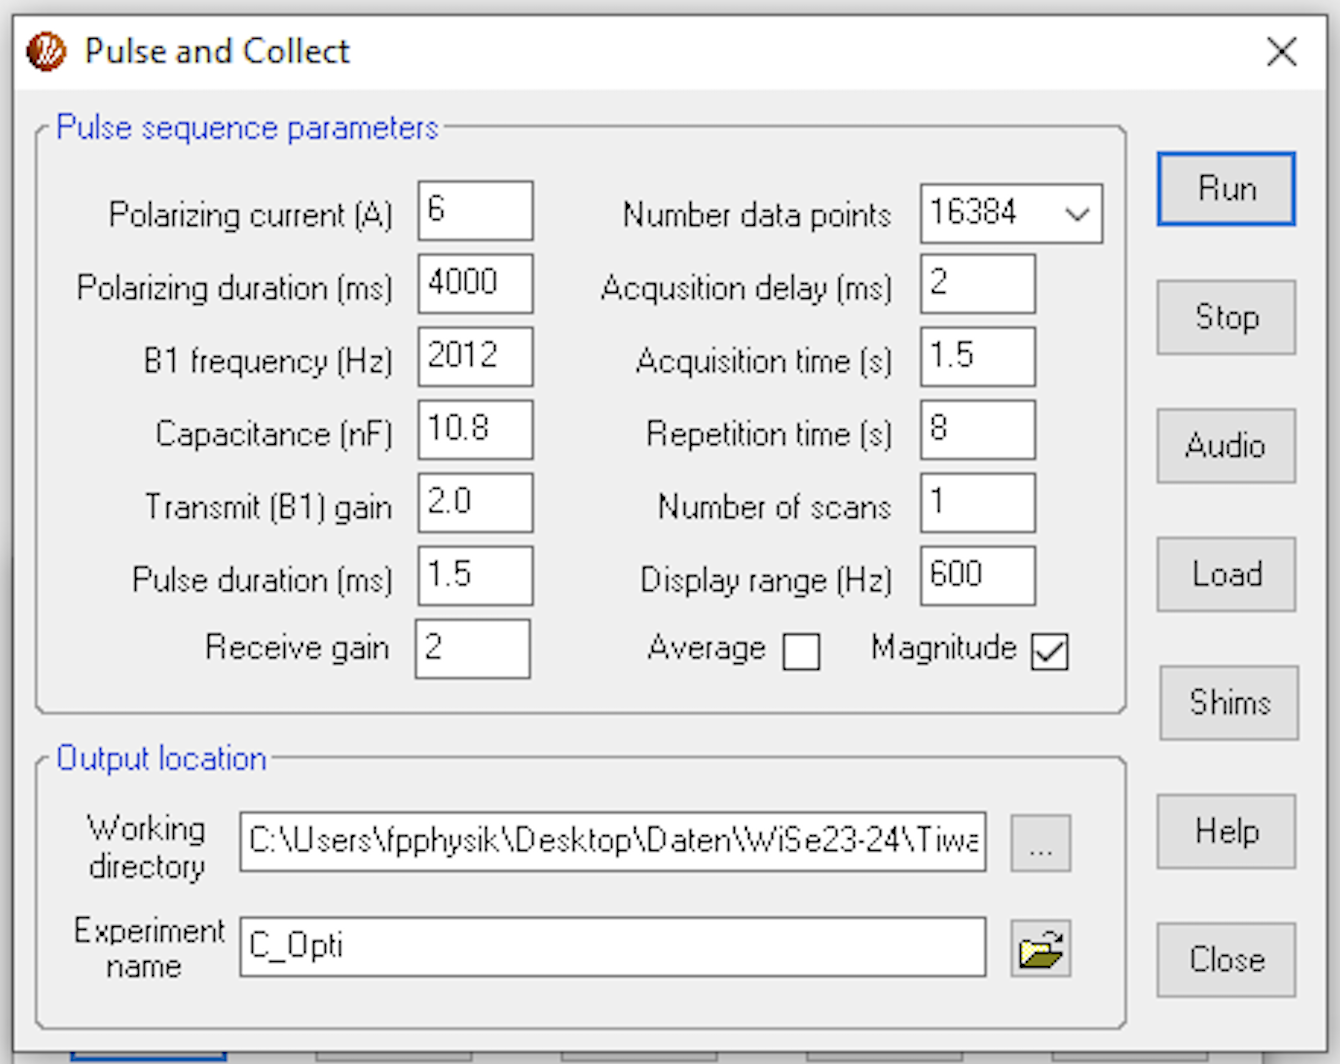
\includegraphics[width=7cm]{Bilddateien/5/C_Abtastparameter.png}
                \caption{Messparameter zur optimierten $B_1$ Dauer.}
                \label{fig:5.1:B1OptiParameter}
            \end{figure}

        \subsubsection*{Optimierung der $B_1$ Pulsdauer}\label{subsubsec:5:B1PulsdauerOptimierung}
            Um eine Amplitudenmaximierung des Spektrums weiter zu verfolgen, optimieren wir die $B_1$ Pulsdauer $t_{B_1}$. Diese stellt allgemein als ein Parameter der Auslenkung der Nukleonenmagnetisierungen gegen ihre Ruhelage im Magnetfeld eine Möglichkeit der Amplitudenmaximierung dar. Im Speziellen wählen wir für einen $\pi/2$ Puls die Dauer hin zum ersten Maximum der Kurve, die $\pi$ Pulslänge ergibt sich dann durch die Dauer zum ersten Minimum, da die Nukleonenmagnetisierung hier umgekehrt wird und eine minimale Präzession stattfindet. 
            \begin{figure}[H]
                \centering
                \begin{subfigure}[t]{0.45\textwidth}
                    \centering
                    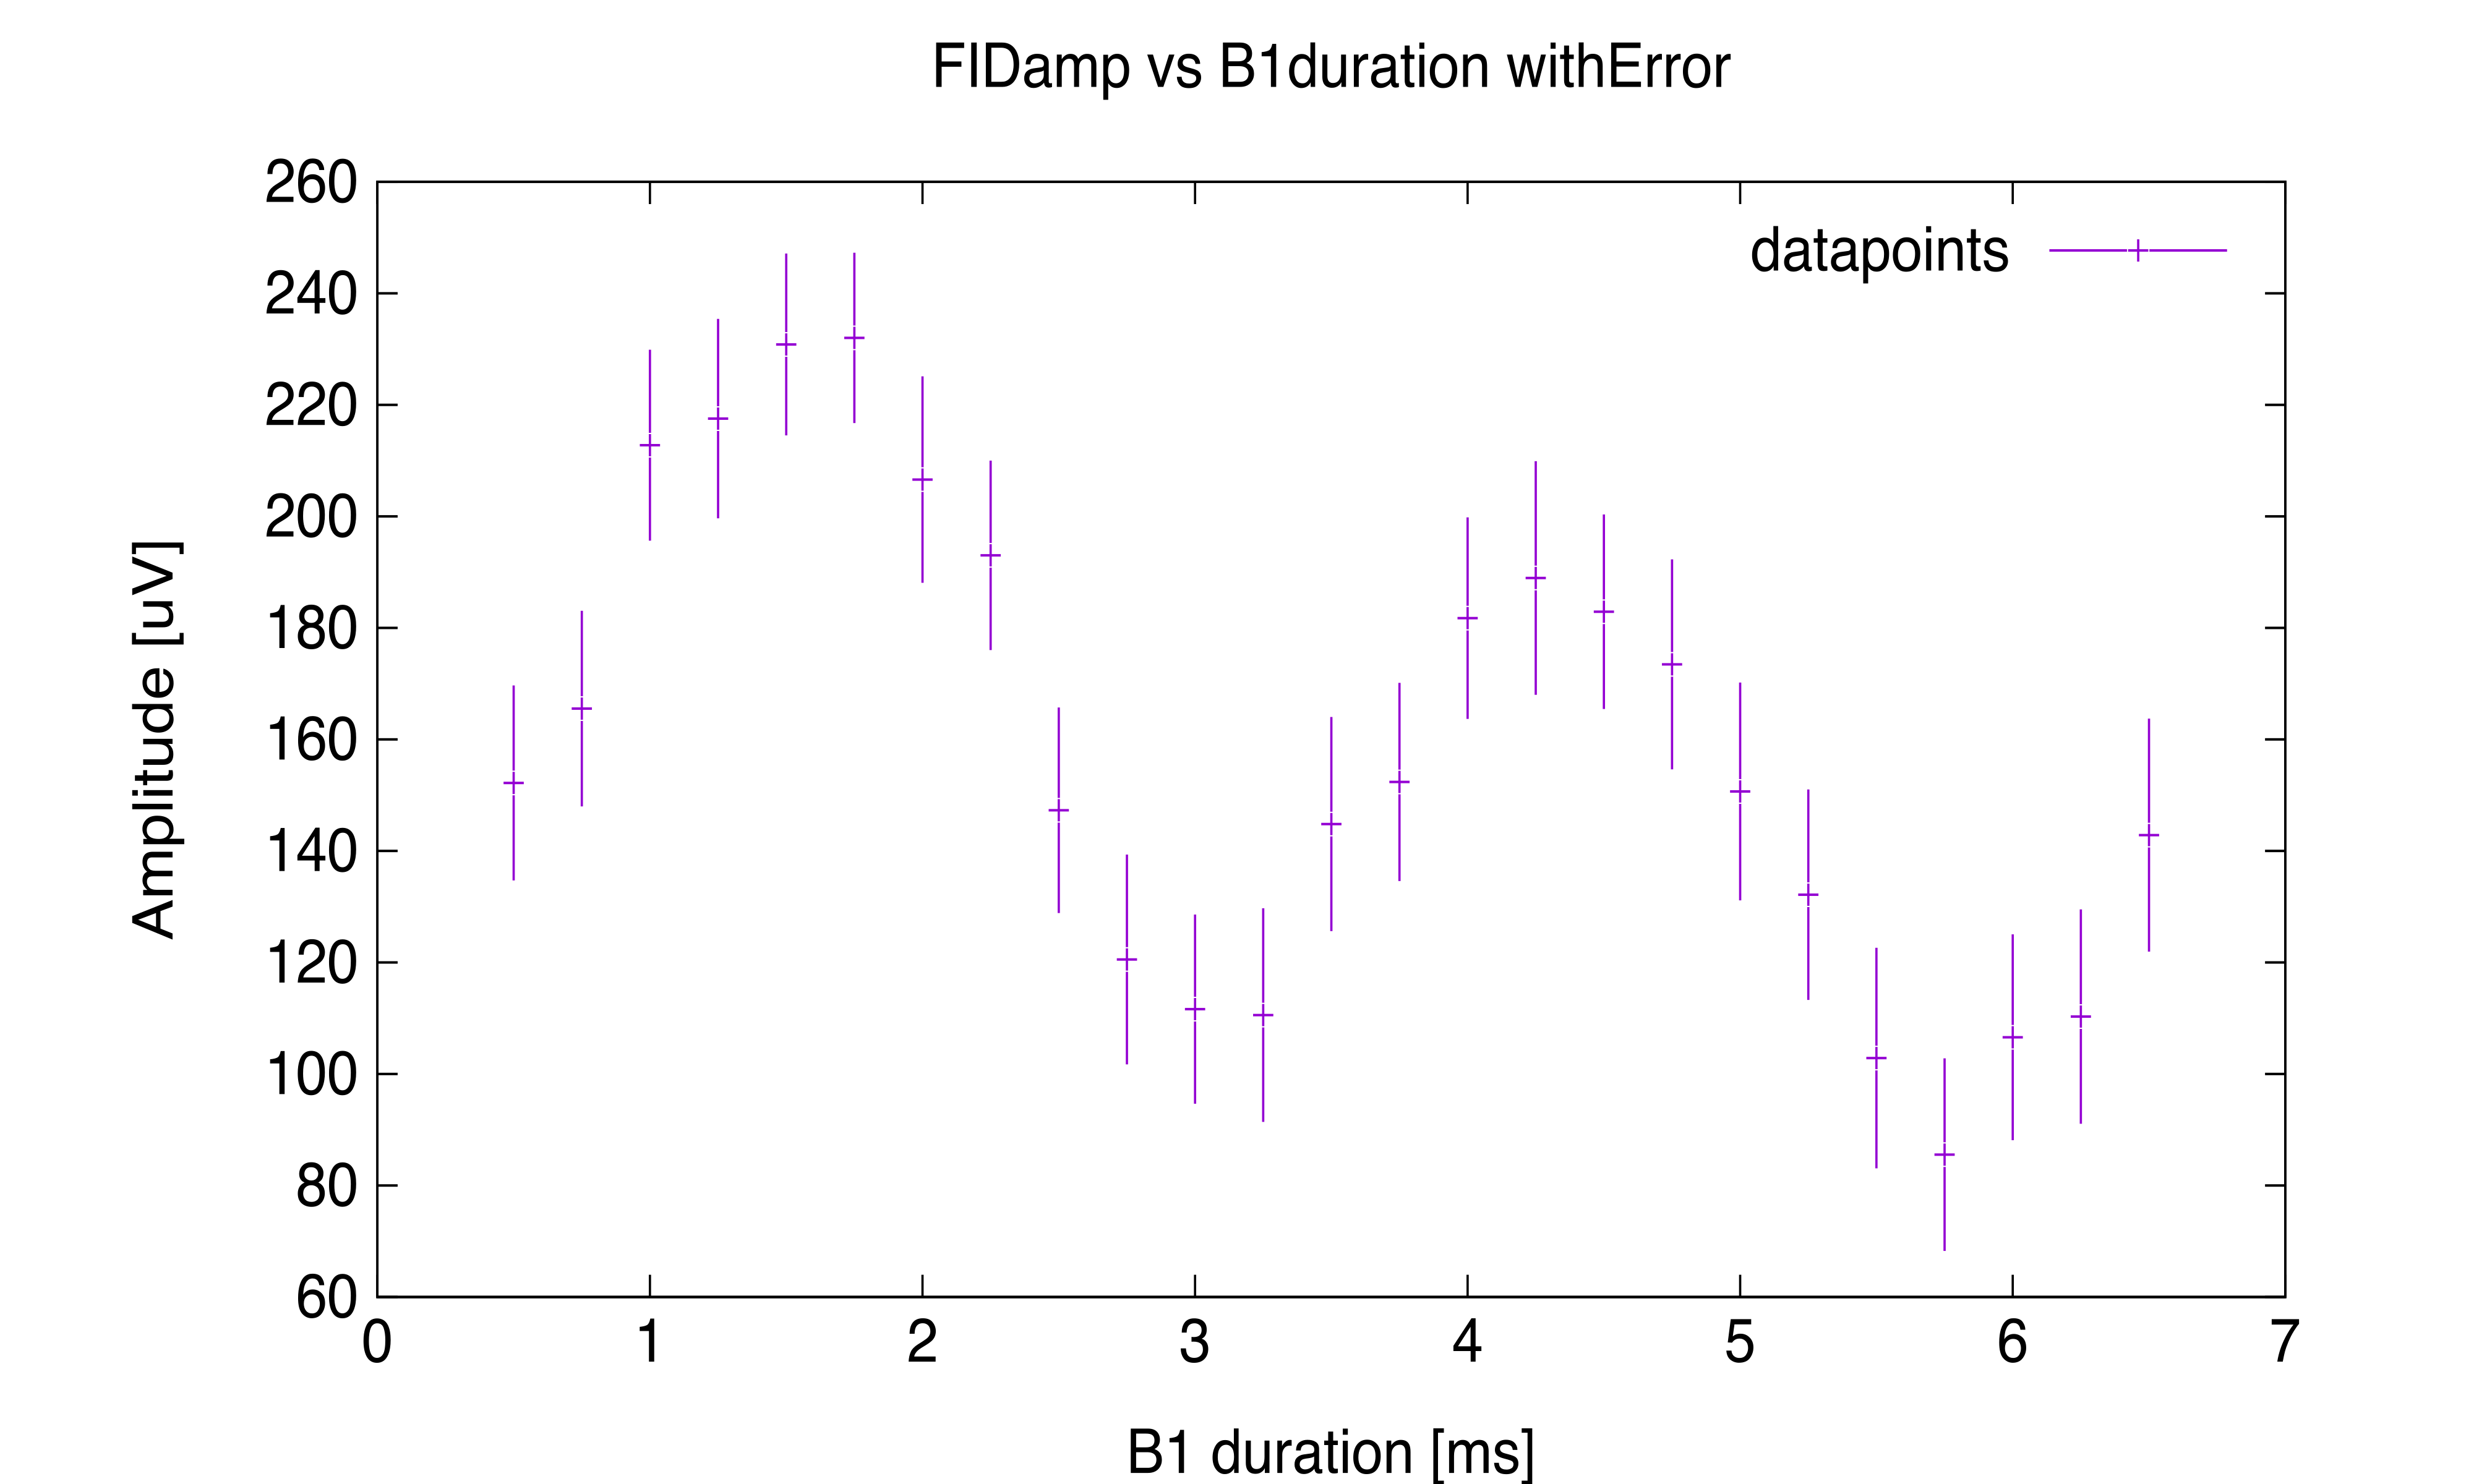
\includegraphics[width=6cm]{Bilddateien/5/B1DurationFast_FIDamp_vs_B1duration_withError.png}
                    \caption{Messung der FID-Amplitude mit Fehlerbalken in Abhängigkeit der B1-Dauer.}
                    \label{fig:5:FastFIDampVsB1durationWithError}
                \end{subfigure}
                \
                \begin{subfigure}[t]{0.45\textwidth}
                    \centering
                    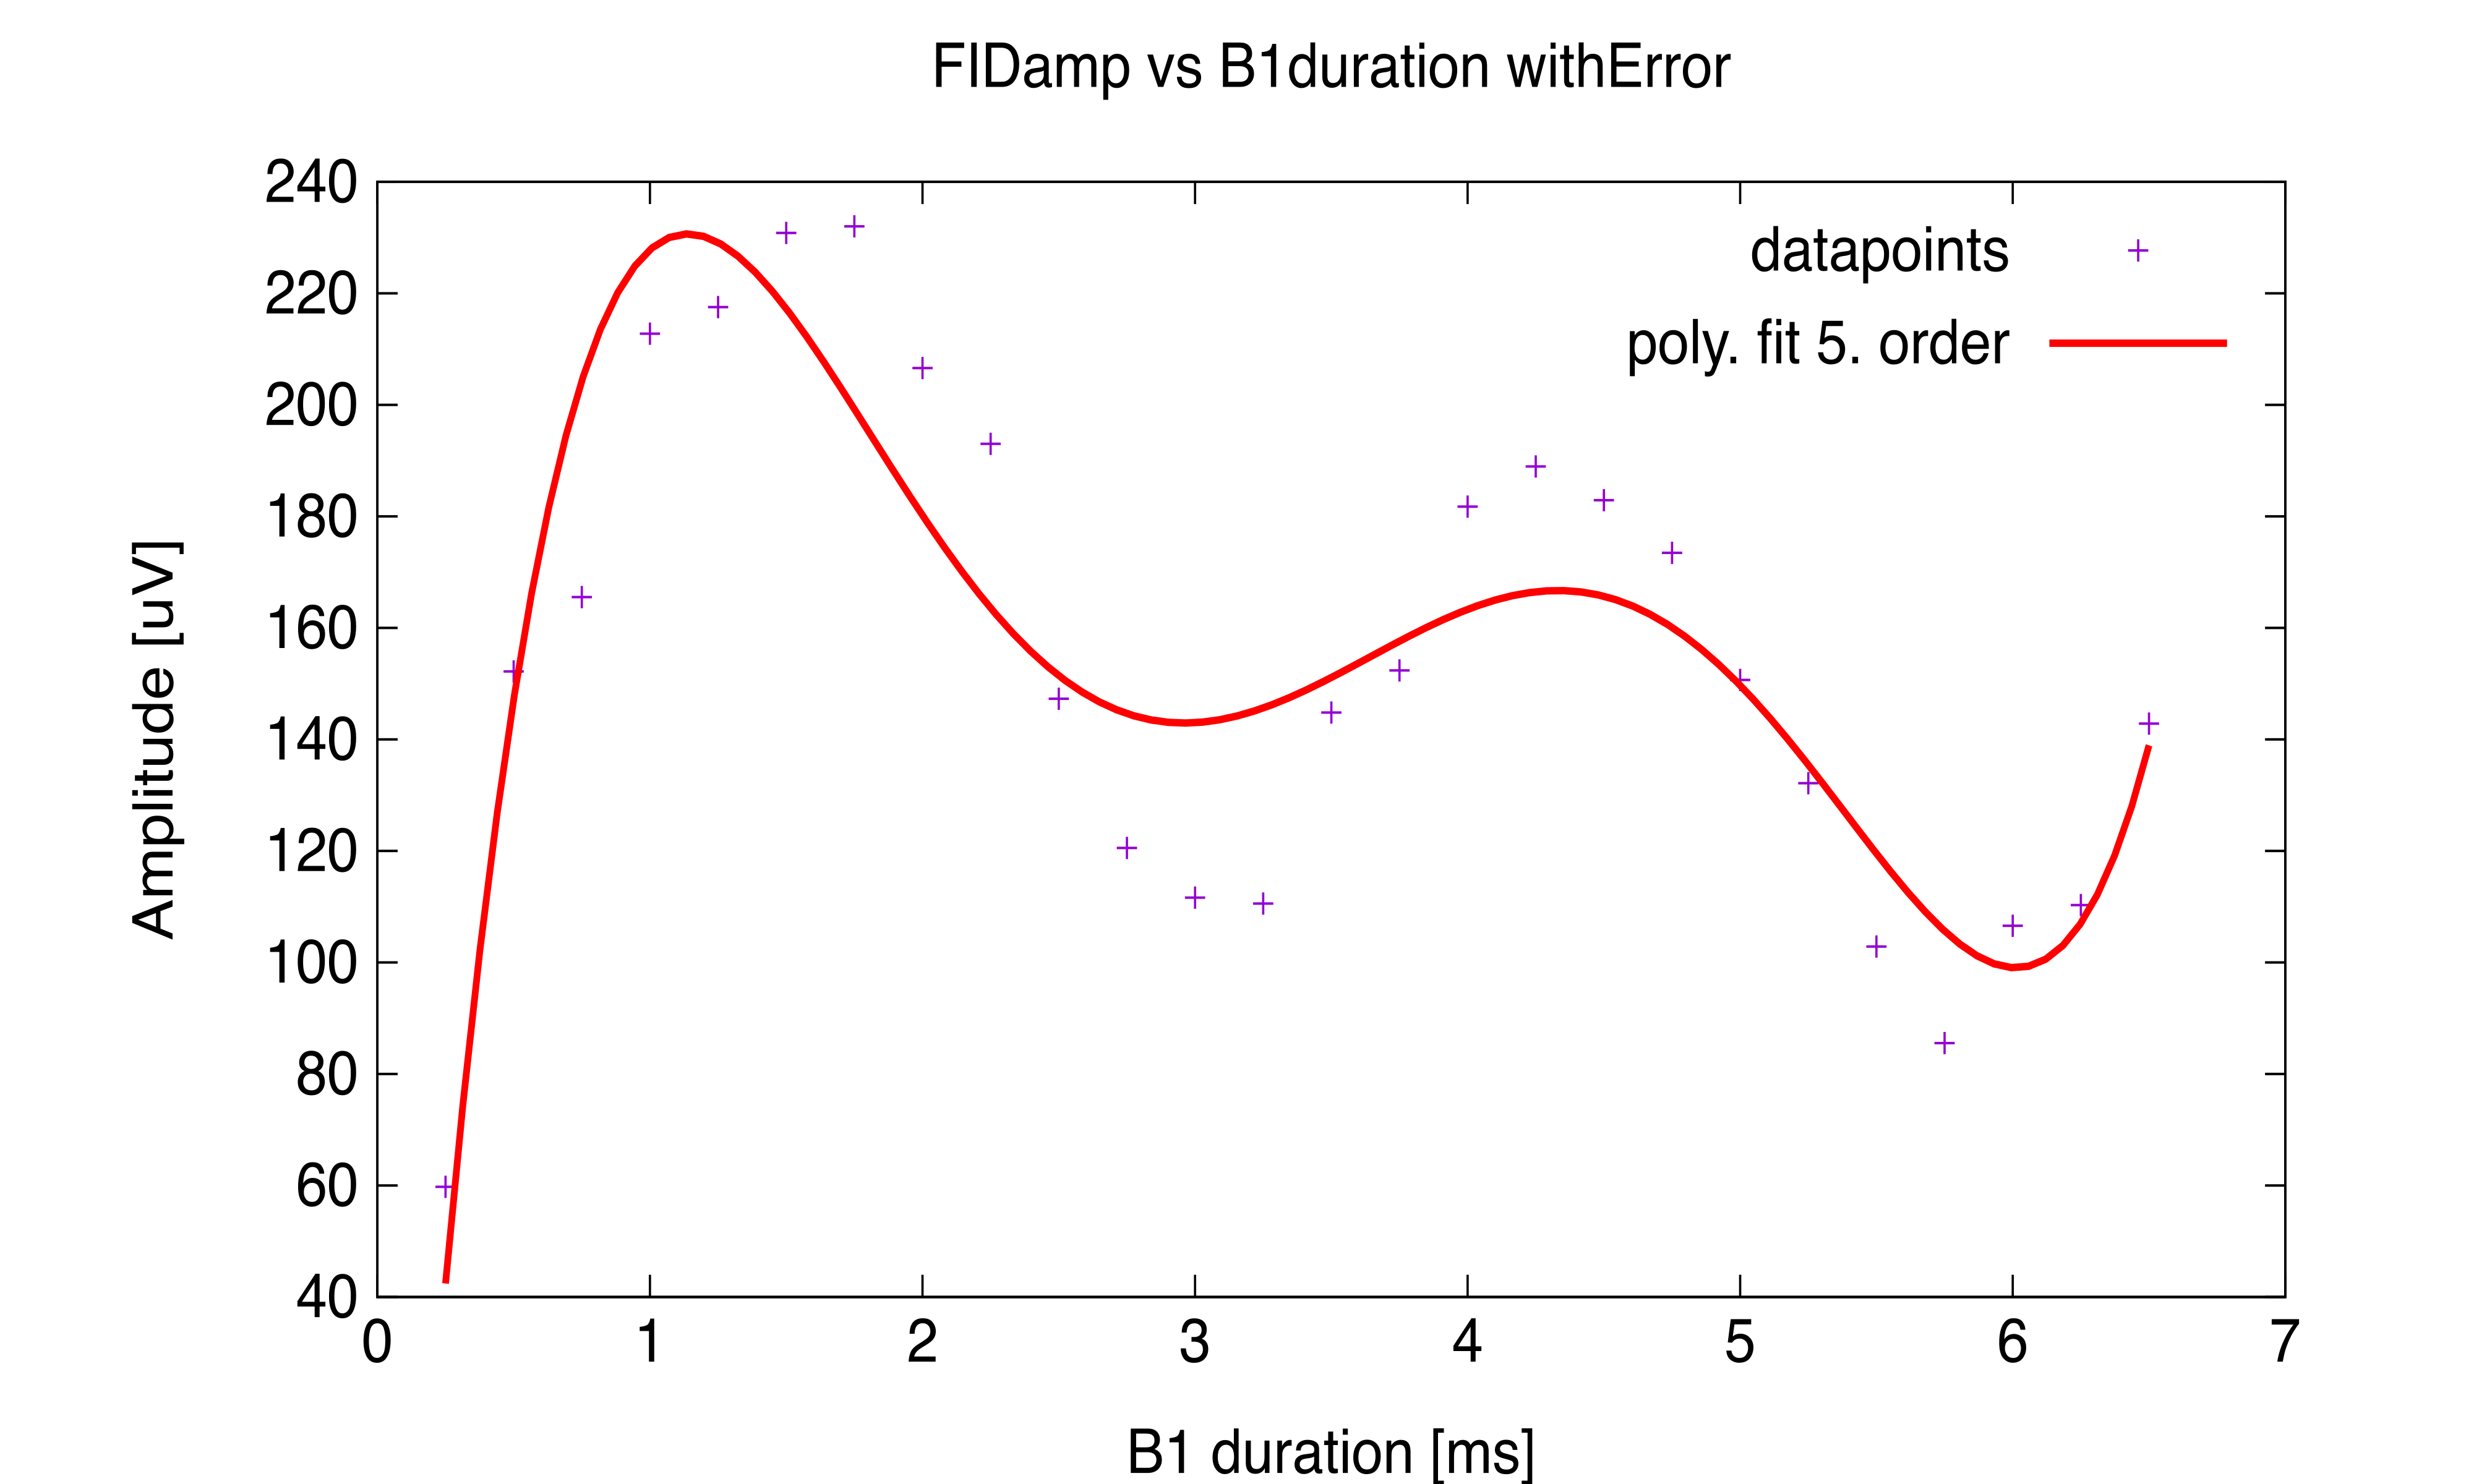
\includegraphics[width=6cm]{Bilddateien/5/B1DurationFast_FIDamp_vs_B1duration_withError_poly.png}
                    \caption{Messung der FID-Amplitude in Abhängigkeit der B1-Dauer mit polynomialer Kurvenanpassung neunter Ordnung.}
                    \label{fig:5:FastFIDampVsB1duration}
                \end{subfigure}
                \caption{Messung der FID-Amplitude in Abhängigkeit der B1-Dauer.}
            \end{figure}
            Obwohl wir mithilfe einer polynomialen Kurvenanpassung eine mögliche Approximation des Kurvenverlaufes erhalten, ist aufgrund unbekanntem theoretischen Hintergrund eine funktionelle Interpretation der Daten nicht fundiert möglich. Die Unsicherheiten der Polynom effizienten liegt des weiteren zwischen $20$ und $30$ Prozent. \\

            Dargestellt in Tabelle \ref{tab:5:OptiB1Duration} sind die aus Abbildung \ref{fig:5:FastFIDampVsB1durationWithError} erhaltenen ersten Maximal- und Minimalargumente der iterativen Amplitudenmessung. Dabei ist die am Computer eingestellte Abtastbreite $\delta t = 0.25\si{\ms}$ ein Maß ihrer Unsicherheit.

            \begin{table}[H]
                \centering
                \begin{tabular}{c|cc}
                    Puls & $t$ in $\si{\ms}$ & $A$ in $\si{\micro\volt}$ \\
                    \hline\hline
                    $\pi/2$ & $1.75(25)$ & $232.01(1527)$ \\
                    $\pi$ & $3.25(25)$ & $110.56(19157)$
                \end{tabular}
                \caption{Max- und minimale Argumente der iterativen Amplitudenmessung zur Bestimmung der optimalen $B_1$ Pulsdauer für $\pi/2$ und $\pi$ Pulse.}
                \label{tab:5:OptiB1Duration}
            \end{table}
            Dies bringt uns insgesamt auf eine Parameterwahl wie in Abbildung \ref{fig:5.2:Abtastparameter} dargestellt.
            \begin{figure}[H]
                \centering
                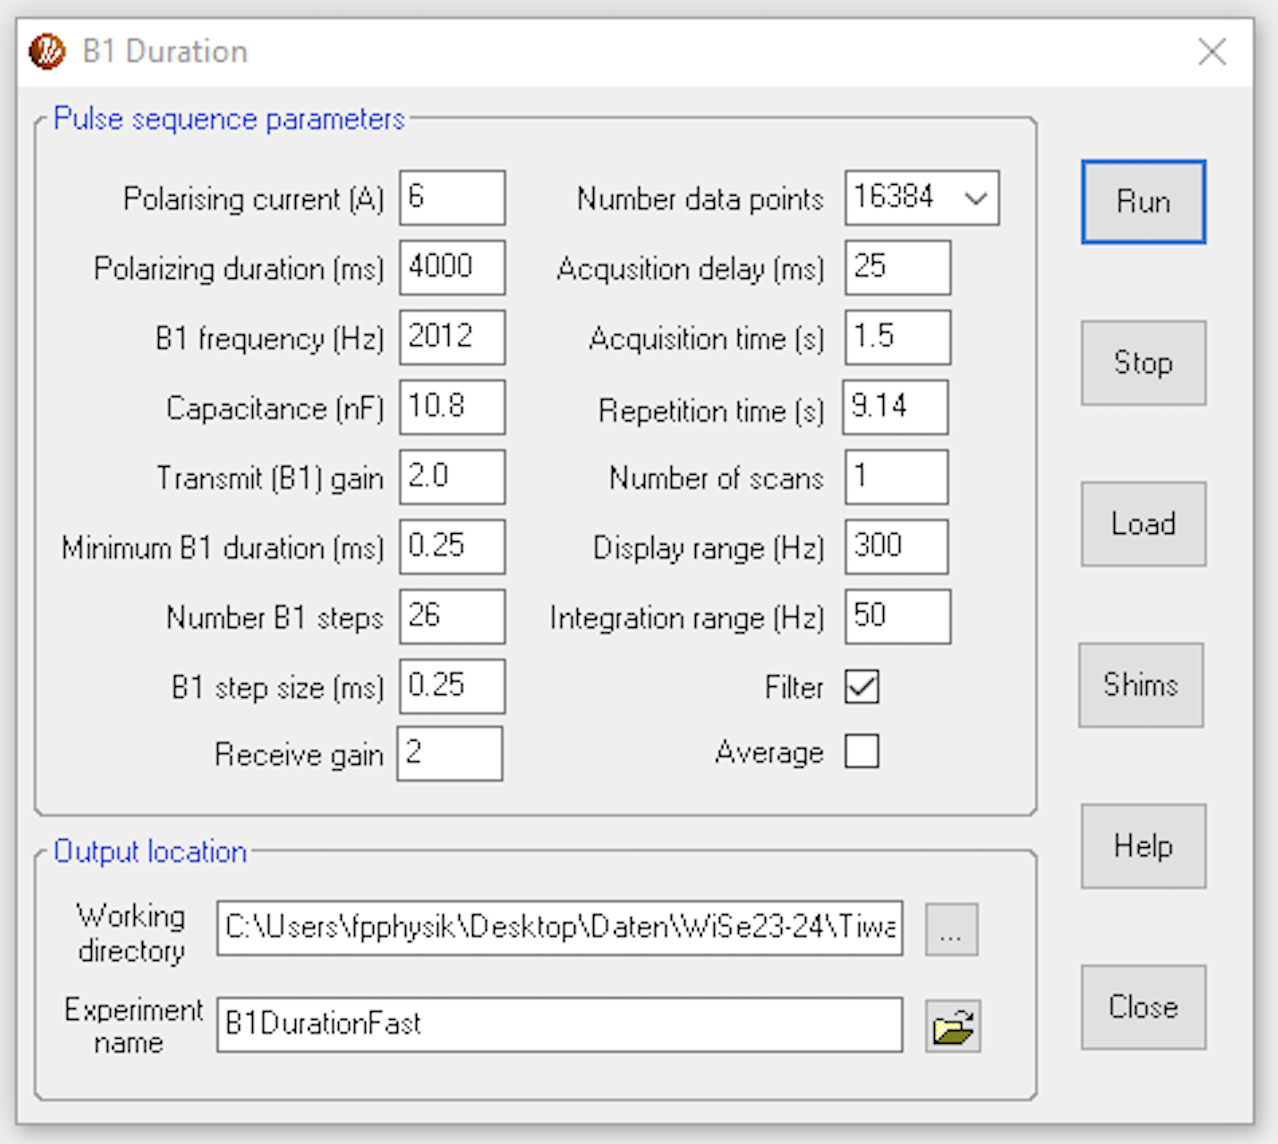
\includegraphics[width=7cm]{Bilddateien/5/B1Duration_Abtastparameter.png}
                \caption{Abtastparameter zur Bestimmung der optimalen $B_1$ Pulsdauer.}
                \label{fig:5.2:Abtastparameter}
            \end{figure}

        \subsubsection*{Anwendung der optimierten $B_1$ und $C$ Parameter}
            Unter Verwendung der obig bestimmten Parameter $C$ und $t_{B_1}$ erhalten wir das Spektrum \ref{fig:5:OptiSpectrum}. Es besitzt bereits eine zu Abbildung \ref{subfig:5:OptiCSpectrum} ähnliche Form, da effektiv lediglich $t_{B_1}$ um $0.2\si{\milli\second}$ erhöht wurde. Dies führt offen erkennbar dennoch zu einem höheren Amplitudenmaximum.
            \begin{figure}[H]
                \centering
                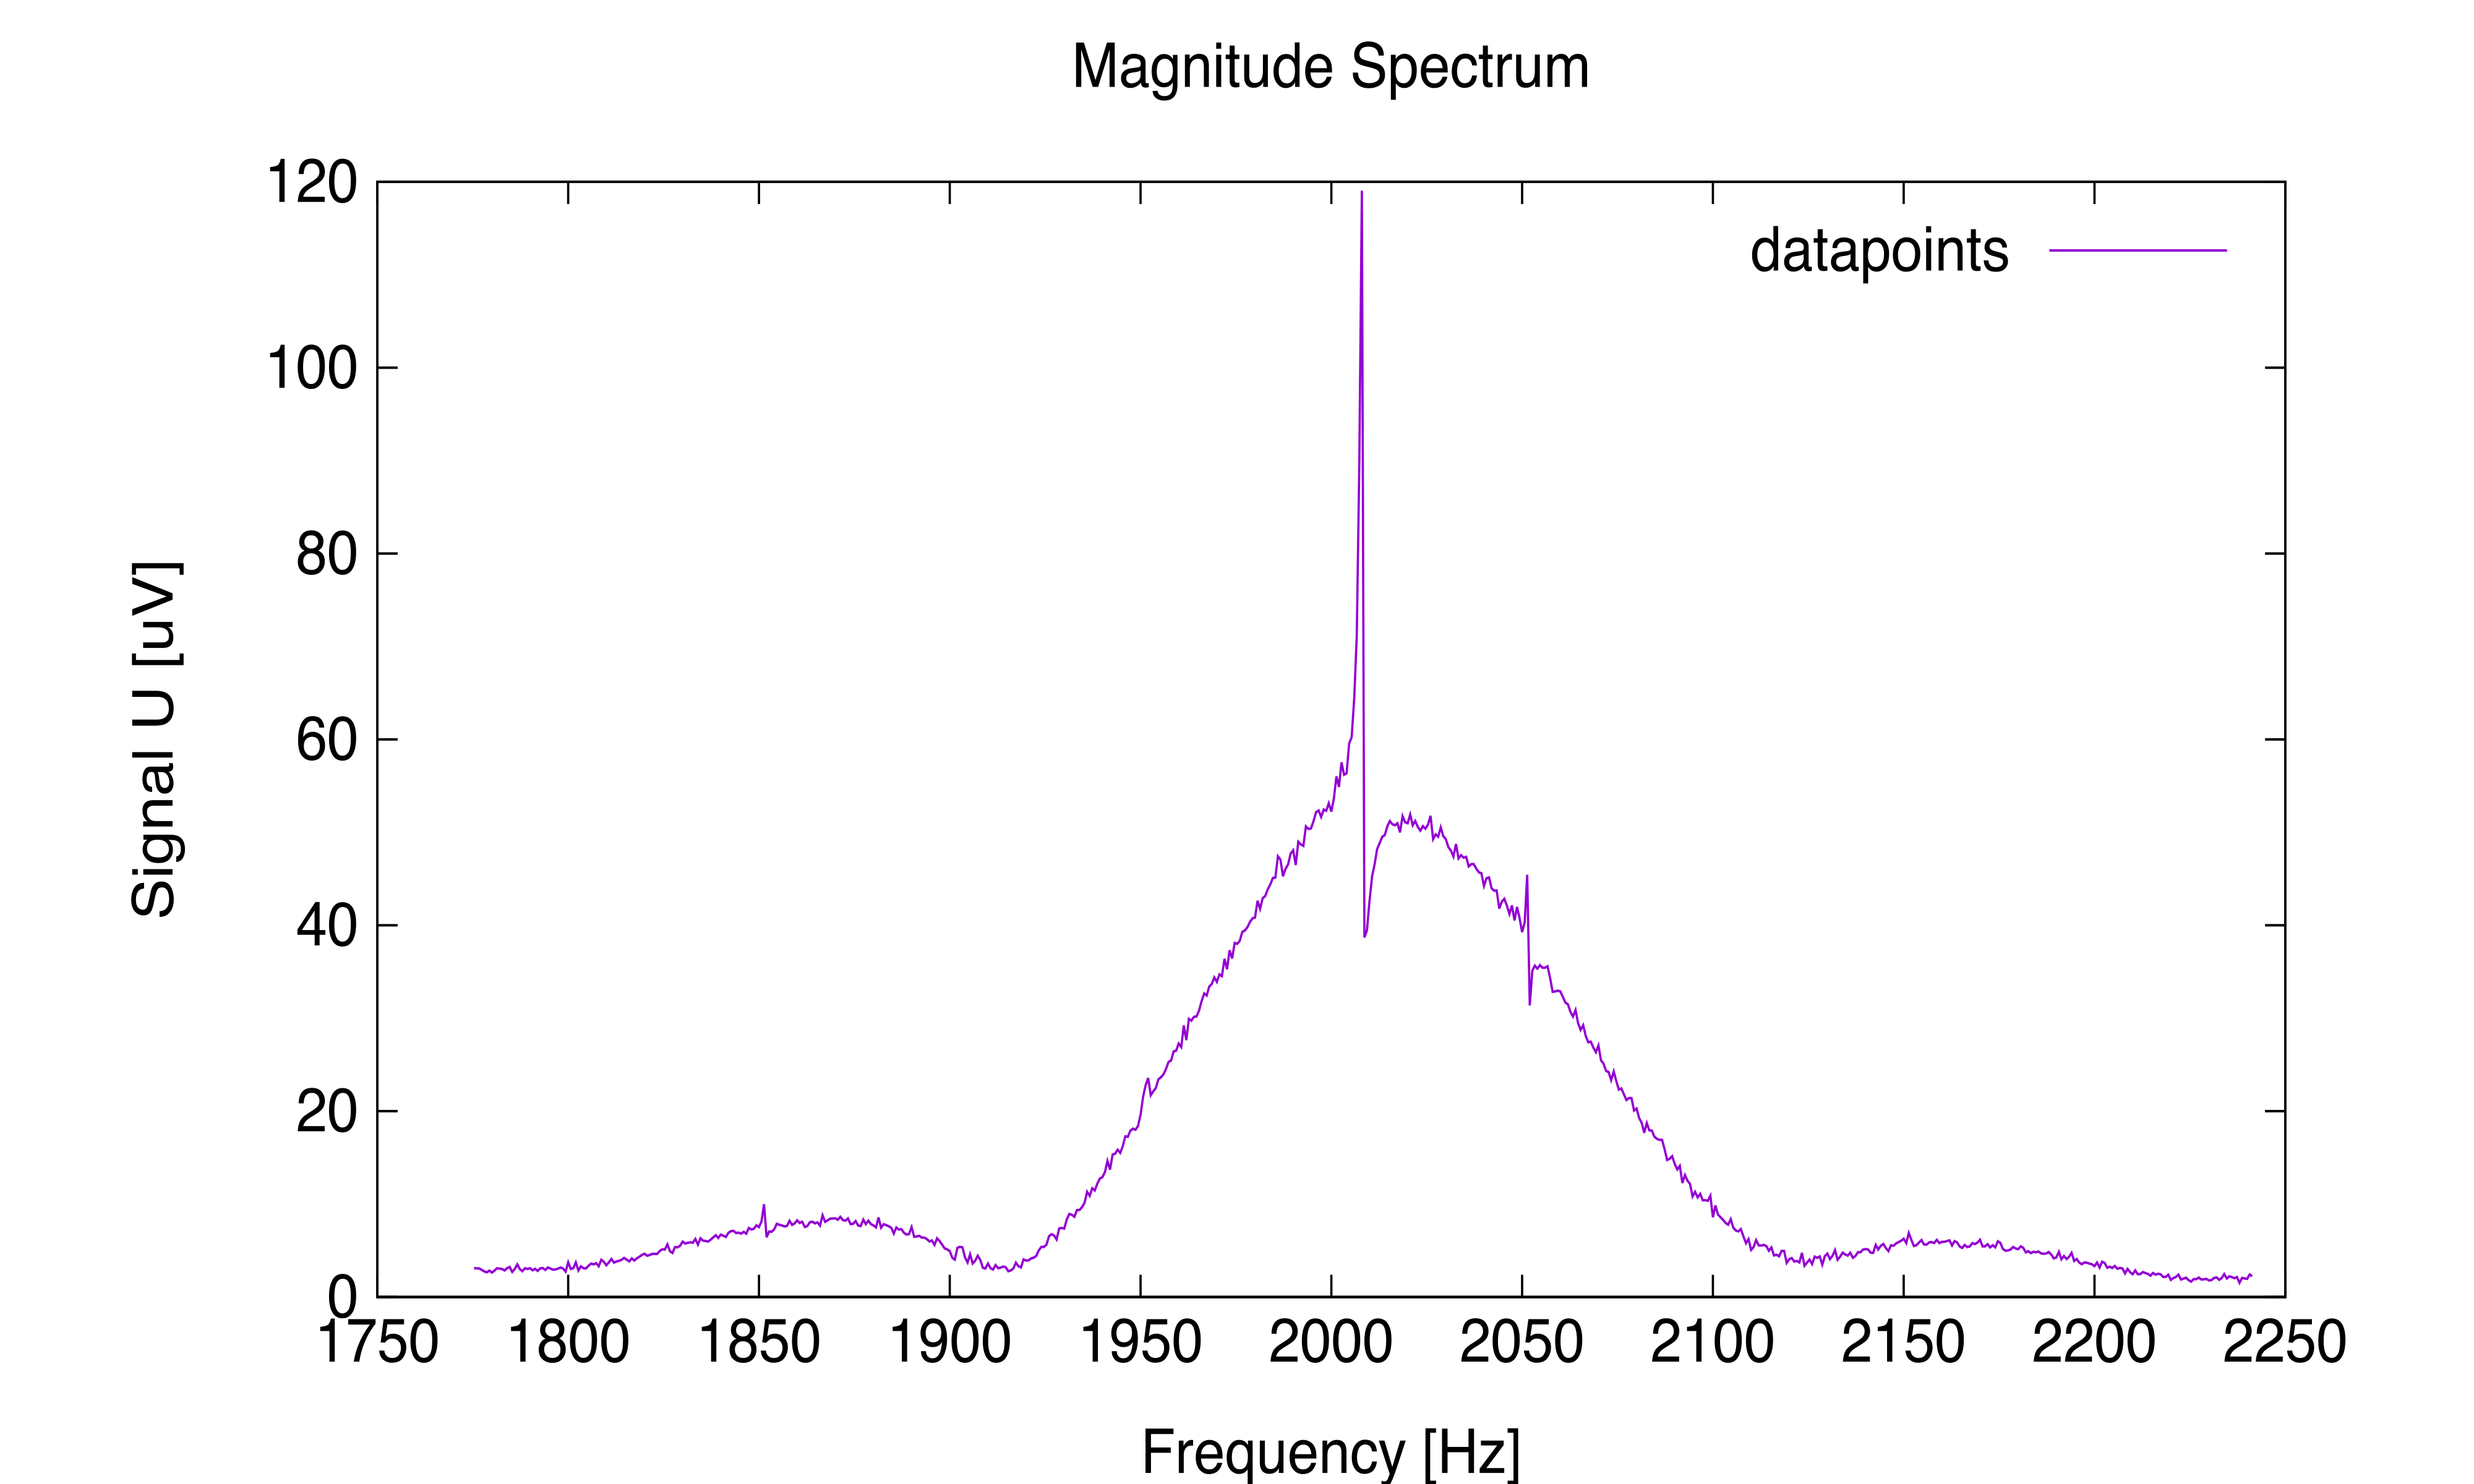
\includegraphics[width=11cm]{Bilddateien/5/B1_Opti_Spectrum.png}
                \caption{Spektrum mit optimierten Parametern $C$ und $t_{B_1}$.}
                \label{fig:5:OptiSpectrum}
            \end{figure}


    % \bibliography{../Literatur.bib}
\end{document}